\documentclass[twoside,12pt]{article}

%Kindle touch setup
\ifx\kindle y
\usepackage[papersize={3.3in,4.4in},hmargin=0.1in,vmargin={0.1in,0.1in}]{geometry}
\fi

%Phone setup
\ifx\phone y
\usepackage[papersize={3.24in,5.76in},hmargin=0.1in,vmargin={0.1in,0.1in}]{geometry}
\fi

\usepackage[spanish]{babel}
\usepackage{graphicx}
\usepackage{float}
\usepackage[utf8]{inputenc}
\usepackage{xfrac}
\usepackage{hyperref}
\hypersetup{
    colorlinks,
    citecolor=black,
    filecolor=black,
    linkcolor=black,
    urlcolor=black
}
\usepackage{amsmath}

\newcommand{\Sim}{$\sim$}
\renewcommand{\deg}{$^{\circ}$}

\usepackage{siunitx}
\sisetup{quotient-mode = fraction}
\sisetup{fraction-function=\sfrac}
\sisetup{range-phrase = -}

\setlength\parindent{0pt}
\date{}
\author{Israel, Kris, Paco y Ana}

\title{Recetario}

\begin{document}
\maketitle

\tableofcontents

\newpage
\section{Desayunos}
\subsection{Buttermilk pancakes}

\begin{itemize}
\item 1 $\sfrac{1}{4}$ tazas de harina
\item 1 huevo
\item 1 $\sfrac{1}{4}$ tazas de buttermilk (como substituto  de  $\sfrac{3}{4}$ a 1 tazas de leche\footnote{Dependiendo de que tan gorditos los quieres} con 2 cucharadas de vinagre y dejar por 5 min)
\item $\sfrac{1}{4}$ de taza de azucar
\item $\sfrac{1}{4}$ de taza de aceite
\item 1 cucharadita de polvo para hornear
\item 1 cucharadita de bicarbonato
\item 1 cucharada de vainilla
\end{itemize}

\subsection{Chilaquiles rojos}\label{chilaquiles-rojos}

Basada en: \href{https://www.youtube.com/watch?v=I8xJOKFjDF4}{CHILAQUILES ROJOS - Vicky Receta Facil} \\

\underline{Ingredientes}

\textbf{Salsa}
\begin{itemize}
\item 4 jitomates
\item 3 chiles huajillo
\item Chile de arbol al gusto
\item Sal al gusto
\item 1 diente de ajo
\item 1 rebanada de cebolla
\item 1 cubo de consome de pollo
\end{itemize}

\textbf{Totopos}
\begin{itemize}
\item $\sfrac{1}{2}$ kg de tortilla
\item Aceite vegetal
\end{itemize}

\textbf{Para acompañar}
\begin{itemize}
\item Crema
\item Queso seco
\item Cebolla con limon
\end{itemize}

\underline{Instrucciones}

\textbf{Salsa}
\begin{enumerate}
\item Cocer los tomates hasta que reviente
\item Remover las semillas del chile huajillo. 
\item Cocer todos los chiles hasta que se aguaden.
\item Licuar todo
\item Hervir por \Sim10-15min. Agregar agua si es necesario.
\end{enumerate}

\textbf{Totopos}
\begin{itemize}
\item Dejar las tortillas afuera por \Sim 1dia para que se sequen
\item Cortar en 6
\item Poner en aceite caliente hasta que se doren.
\item Dejar escurrir.
\end{itemize}

\textbf{Chilaquiles}
\begin{itemize}
\item Hacer la salsa.
\item Hacer los totopos. De preferencia hacerlos hasta que ya este lista la salsa.
\item Bañar los totopos con las salsa y revolver bien en un sartén.
\item Cubrir con crema, queso y cebolla desflemada. 
\end{itemize}


\subsection{Chilaquiles verdes}\label{chilaquiles-verdes}

Basada en: \href{https://www.youtube.com/watch?v=CcuHrqMZOFU}{CHILAQUILES VERDES - Vicky Receta Facil} \\

Igual que chilaquiles rojos (\ref{chilaquiles-rojos})  excepto la salsa.

\underline{Ingredientes}

\textbf{Salsa}
\begin{itemize}
\item 300 gr de tomate verde
\item \Sim 6 ramitas de cilanto
\item 4 chiles verde (o al gusto)
\item 1 rebanada de cebolla
\item 1 rama de epazote fresco
\item 1 diente de ajo
\item 1 cubo de caldo de pollo
\item Sal al gusto
\end{itemize}


\underline{Instrucciones}

\textbf{Salsa}
\begin{enumerate}
\item Cocer los tomates y el chile hasta que cambiend de color
\item Licuar todo
\item Cocer por \Sim 10min. Agregar agua si es necesario
\end{enumerate}



\section{Recetas mexicanas}
\subsection{Rajas con queso}

\underline{Ingredientes}
\begin{itemize}
\item 8 chiles poblanos
\item $\sfrac{3}{4}$ de taza de elote
\item 2 rebanadas de cebolla
\item 4 cucharadas de crema
\item 1 cubito de caldo de pollo.
\item 2 cucharada de aceite
\item 70 gr de queso rayado
\end{itemize}

\underline{Instrucciones}
\begin{enumerate}
\item Preparar los chiles
\begin{enumerate}
\item Quemar
\item Sudar
\item Pelar
\item Quitar semillas
\item Cortar
\end{enumerate}
\item Sofreir la cebolla, rajas y elote en aceite.
\item Agregar el cubo de pollo y la crema, y dejar que hierva un par de minutos.
\item Agregar queso rayado
\end{enumerate}

\subsection{Tamales rojos}

\underline{Ingredientes (\Sim 16 tamales)}

\begin{itemize}
\item \Sim 30hojas de maíz secas
\end{itemize}

\textbf{Carne}
\begin{itemize}
\item \Sim 1 kg de carne de puerco
\item 1 diente de ajo
\item 5 pimientas negras
\item 4 hojas de laurel
\item \Sim $\sfrac{1}{4}$ de cebolla
\item \Sim 1 chucharada de sal
\end{itemize}

\textbf{Salsa}

\begin{itemize}
\item \Sim 1 cucharadita de sal
\item 12 chiles guiajillos o anchos o combinación.
\item \Sim 10 chiles de árbol
\item \Sim 2 dientes de ajo
\item 2 clavos
\item 8 pimientas negras
\item \Sim $\sfrac{1}{4}$ de cebolla pequeña
\item 2 jitomates
\item $\sfrac{1}{4}$ de cucharaditas de comino
\item $\sfrac{1}{2}$ cucharadita de orégano
\end{itemize}

\textbf{Masa}

\begin{enumerate}
\item 4 tazas de Maseca pra tamal
\item 3 tazas de consomé de pollo
\item 2 cucharadita de sal
\item 2 cucharaditas de polvo para hornear
\item 1 $\sfrac{1}{3}$ tazas de manteca de puerco o vegetal
\end{enumerate}

\underline{Instrucciones}

\textbf{Carne}

\begin{enumerate}
\item Cocer en en olla a presión con el resto de los ingredientes (20 min después de que comience a bambolear).
\item Desmenuzar
\end{enumerate}

\textbf{Salsa}

\begin{enumerate}
\item Cocer los tomates hasta que revientes
\item Remover semillas de chiles guajillos.
\item Cocer los chiles por \Sim 5min.
\item Licuar todo
\end{enumerate}

\textbf{Masa}

\begin{enumerate}
\item Revolver la manteca hasta que este suave
\item Agregar el resto de los ingredientes hasta que la masa este esponjosa
\item Si hace falta, agregar un poco de agua hasta que la masa se pueda untar facilmente
\end{enumerate}

\textbf{Tamales}

\begin{enumerate}
\item Poner a remojar las hojas en agua caliente hasta que esten aguaditas.
\item Preparar carne, salsa y masa.
\item En una hoja, untar una capa de masa, luego un caminito de carne y un caminito de salsa.
\item Doblar la hoja en tres y luego doblar el fondo.
\item Poner agua y hojas en el fondo de un vaporea.
\item Acomodar los tamales boca arriba (de preferencia completamente lleno, apretados).
\item Clavar hojas de tamal a los lados y tapar.
\item Cocer a fuego bajo for 1:45 horas.
\end{enumerate}

\underline{Notas}

Basada en Vicky Receta Fácil \href{https://www.youtube.com/watch?v=y-_ozklQH7w}{link} (\url{fuentes/tamales_rojos-Vicky_Receta_facil.mp4}). Masa según el empaque de Maseca para Tamal.

\subsection{Tortillas}

\underline{Ingredientes (4-6 tortillas)}\\
Masa (de \hyperref[receta:masa-maiz]{nixtamal} o \hyperref[receta:masa-maseca]{maseca})\\

\underline{Instrucciones}
\begin{enumerate}
\item Precalentar comal a fuego alto. De preferencia uno grueso para que el tenga una temperatura uniforme.
\item Mezclar maseca y agua
\item Si es necesario, agregar un poco de maseca. Debe de quedar lo más humeda posible pero que siga siendo manejable.
\item Aplanar con tortillera y bolsa de plastico delgado (de la sección de frutas y verduras).
\item Dejar en el comal por \SIrange{15}{30}{sec}, hasta que cambie ligeramente de color, y voltear.
\item Dejar en el comal por \SIrange{90}{120}{sec}, hasta que se vean partes ``seca'' o ``bombitas'', y voltear.
\item Esperar a que se infle y dejar por \SI{15}{s} más. Si no se infla sóla, una presión suave con la mano ayuda.
\item Sacar del comal.
\end{enumerate}


\subsection{Frijoles refritos}
\label{sec:frijoles-refritos}

\textbf{Ingredientes}
\begin{itemize}
\item \sfrac{1}{2} kilo de frijoles
\item 3 litros de agua
\item 2 cucharadas de sal?
\item \sfrac{1}{2} taza de aceite?
\item 5 chiles verdes
\item \sfrac{1}{4} de cebolla en rodajas
\end{itemize}

\textbf{Instrucciones}
\begin{enumerate}
\item Limpiar y lavar los frijoles
\item Dejar remojando una noche con toda el agua
\item Cocer a fuego medio hasta que el borde del agua llegue al borde de los frijoles
\item Calentar el aceite y apagar cuando humee ligeramente.
\item Echar los chiles y la cebolla. ¡Con cuidado que salpica!
\item Retirar cuando deje de burbujear.
\item Prender a fuego bajo
\item Agregar los frijoles y machacar, poco a poco.
\item Agrega agua de los frijole hasta que tenga la consistencia deseada.
\item Poner los chiles de vuelta y apagar cuando hierva  
\end{enumerate}

\subsection{Chiles rellenos}
\textbf{Ingredientes}
\begin{itemize}
\item 1 chile poblano
\item 2 huevos
\item $\sim$100 gr de queso para derretir (e.g. Oaxaca, Chihuahua, asadero)
\item Harina (para espolvorear)
\item Dos cucharadas de aceite
\end{itemize}

\textbf{Instrucciones}
\begin{enumerate}
\item Poner el chile al fuego hasta que este blandito y la mayor parte de la piel este quemada.
\item Envolverlo con pl\'astico y dejar que se enfr\'ie.
\item Remover la piel.
\item Hacer una abertura por un lado y rellenar de queso.
\item Espolvorear y cubrir con harina.
\item Batir las dos claras de huevo hasta punto de turron. Cuando este listo, agregar media yema y batir lentamente. Descartar el resto.
\item Cubrir con el turron y fre\'ir. Se empieza por donde esta la abertura pasa sellarlo. Con una espatula poner m\'as turron si se descubri\'o alguna parte.
\end{enumerate}

\textbf{Ingredientes salsa}
\begin{itemize}
\item 4 jitomates cocidos
\item 2 tazas de agua
\item 1 cuadrito de caldo de pollo (11 gr)
\item \sfrac{1}{4} cuarto de cebolla.
\item 1 cucharadita de ajo molido
\item 1 cucharadita de sal
\item 1 cuacharadita de oregano molido
\end{itemize}

\subsection{Sopa de tortilla}\label{sopa_tortilla}

2 porciones\\
20 min \\


\underline{Ingredientes}
\begin{itemize}
\item 8 tortillas rebanadas en tiras y fritas en aceite
\item 1/2 cebolla
\item 2 dientes ajo
\item 2 tazas de consomé de pollo 
\item 150 gramos queso panela
\item 1 aguacate
\item 8 hojas epazote
\item 4 tomates
\item 2 chiles guajillo 
\item media crema 
\end{itemize}

\begin{figure}[H]
\centering
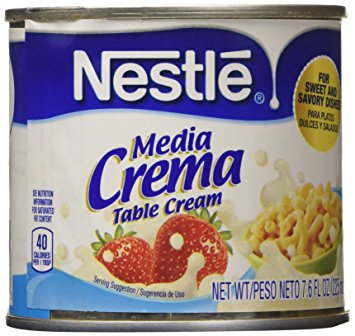
\includegraphics[scale=0.2]{recetas/sopa-de-tortilla/figures/media_crema}
\caption{Media crema. Se encuentra en Target en Baltimore Ave.}
\end{figure}

\underline{Instrucciones}
\begin{enumerate}
\item En una olla con 2 cucharadas de aceite, freír los chiles guajillo cortados en tiras pequeñas y reservar.
\item Licuar los jitomates, cebolla, ajo, 8 tiras de tortilla frita y consomé.
\item Agregar la salsa en la olla con el aceite caliente. Agegar las hojas de epazote.
\item Agregar aproximadamente 1/2 litro de agua a la olla y hervir durante 15 min.
\item Checar si hace falta agua y agregar sal al gusto. La cantidad de agua depende de la consistencia que se quiera alcanzar.
\item En un plato hondo colocar una porción de tortillas fritas y caldo.
\item Decorar con aguacate, panela, crema y tiritas de guajillo.
\end{enumerate}


\begin{figure}[H]
\centering
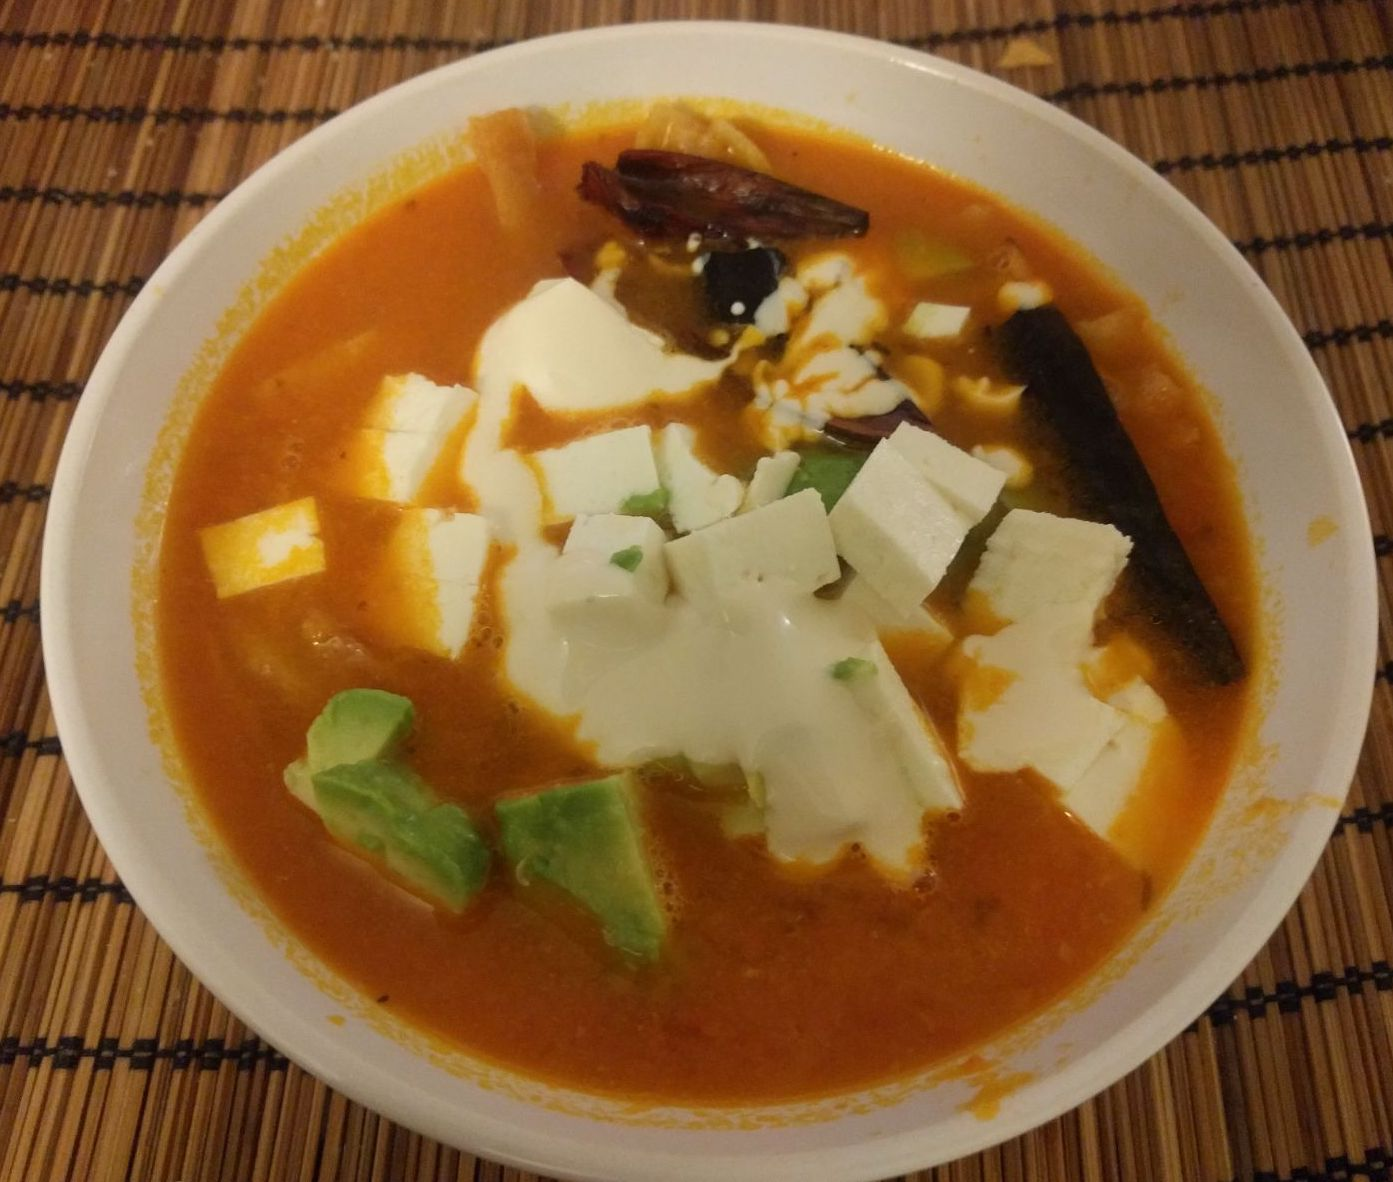
\includegraphics[scale=0.2]{recetas/sopa-de-tortilla/figures/sopa_tortilla}
\caption{Producto final}
\end{figure}


\subsection{Asado de Boda}

\underline{Ingredientes (para taquiza)}
\begin{itemize}
\item 2 naranjas
\item 1 kg de lomo o pierna de cerdo (en cubitos)
\item $\sim 5$ hojas de laurel seco
\item $\sim 4$ clavos
\item $\sim 4$ palitos de canela entera
\item sal y pimienta
\item $\sim 2 $ chiles pasilla secos
\item $\sim 2 $ chiles guajillo secos
\item $\sim 3 $ chiles piquines secos
\item $\sim 3 $ chiles de arbol secos
\item $\sim 2 $ chiles anchos secos
\item $ \frac{1}{2}$ cebolla
\item $\sim 5 $ dientes de ajo
\end{itemize}

\underline{Instrucciones}
\begin{enumerate}
\item Curtir la carne de cerdo en el jugo de las dos naranjas, el clavo, la canela, sal, pimienta, laurel y agregar la cascara de una naranja en rajitas (no usar la cascara de las dos para no amargar mucho la mezcla). Cocinar en slow cooker por $\sim 4 - 5$ hrs. en high.
\item Remojar los chiles en agua caliente hasta que estén suaves.
\item Cuando la carne este lista, separar los cubitos a un lado y colar el jugo que resulta (mezcla de jugo de naranja, jugo de carne y manteca). Enseguida licuar jugo junto con los chiles, cebolla y ajo.  
\item Colar salsa y en una cacerola calentar a fuego lento junto con la carne. Se puede remoler lo que queda en el colador con un poco de salsa y agua para aprovechar los ingredientes al máximo. Se guisa hasta por una hora a fuego muy lento.
\end{enumerate}


\subsection{Pozole verde}

\underline{Ingredientes}
\begin{itemize}
\item $750 \rm{g}$ de nixtamal (maiz)
\item $2 \frac{1}{2}$ ajos
\item $1 \frac{1}{2}$ cebollas
\item $2$ hojas de laurel 
\item $\sim 9$ litros de agua
\item sal de grano
\item $2$ chiles poblanos
\item $2$ chiles jalapeños
\item $1$ chile serrano
\item $250 \rm{g}$ de tomatillo
\item $1 \rm{tz}$ de pepita de calabaza
\item Hierbas verdes (1 ramita de epazote, 6 hojas de espinaca, 1 ramo de cilantro, 1 ramo de perejil y lechuga)
\item $5$ pimientas negras
\item $3$ clavos de olor
\item Manteca de cerdo
\item $1 \rm{cdita}$ de comino
\item $3 \rm{cdas}$ de oregano
\item $1.5 \rm{kg}$ de carne por cada $750 \rm{g}$ de maiz (maciza, cabeza, espinazo, etc.. al gusto de preferencia con hueso para el caldo).
\end{itemize}

\underline{Instrucciones}
\begin{enumerate}
\item Empezando con maiz nixtamalizado, lavar bien y verificar que este bien descabezado el grano. 
\item En agua caliente, se pone a cocer el maiz, dos ajos enteros (mochos para que suelten sabor pero sin pelar), las hojas de laurel y una cebolla grande (mocha o con una cruz para que suelte el sabor).
\item Se parte la carne y se agrega al maiz, junto con un poco de sal.
\item Cocer tomatillos y chiles jalapeños en agua. Por separado, dorar 3 dientes de ajo y media cebolla en manteca. Al final, se reserva la manteca y se licuan la cebolla y el ajo junto con los tomatillos, chiles, pimientas, clavo y dos tazas de agua. 
\item En otra tanda se licuan el resto de las hierbas (epazote, espinaca, cilantro, etc..) junto con las pepitas tostadas $1 \rm{cda}$ de oregano y sal. 
\item Ahora se recuecen las dos salsas en la manteca y la mezcla se deja hervir a fuego lento con un puñito de oregano triturado.
\item Se sacan los ajos, la cebolla y las hojas de laurel del caldo de puerco y se agrega la salsa verde. Se deja a fuego lento y se agrega sal al gusto.
\item Se sirve con chicharron, cebollita picada finamente, rabano, lechuga, tostadas, aguacate y limon.
\end{enumerate}


\subsection{Tacos de canasta}
\label{sec:tacos-de-canasta}

Basada en: \href{https://www.youtube.com/watch?v=kH0nLhOtY2s}{como hacer TACOS DE CANASTA, la receta secreta de los taqueros, \# 456 | Chef Roger} y \href{https://www.youtube.com/watch?v=PoDRiJ3zVmc}{TACOS AL VAPOR ESTILO JALISCO - Alejandra de Nava}\\

También llamados tacos sudados. Aunque son similares a los \href{sec:tacos-al-vapor}{tacos al vapor}, el procedimiento de armado es diferente.\\

\underline{Ingredientes} 

\begin{itemize}
\item \Sim 100 tortillas \footnote{De preferencia recien hechas para que no se rompan. Si son de máquina probablemente necesite llevar tortilla doble.}
\end{itemize}

\textbf{Aceite}
\begin{itemize}
\item 20 chiles guajillos
\item $\sfrac{3}{4}$ de litro de aceite
\item 6 dientes de ajo
\end{itemize}

\textbf{Chicharron prensado}
\begin{itemize}
\item 500gr de chicharron prensado
\item 7 chiles guajillos
\item $\sfrac{1}{4}$ litro de agua
\item $\sfrac{1}{4}$ litro de aceite
\item 2 dientes de ajo
\end{itemize}

\textbf{Puré de papa}
\begin{itemize}
\item 500gr de papa
\item $\sfrac{1}{2}$ cebolla
\item 1 diente de ajo
\item 3 cucharadas de aceite
\end{itemize}

\textbf{Frijoles}
\begin{itemize}
\item 500 gr de rijoles refritos. Ver \href{sec:frijoles-refritos}{receta}.
\end{itemize}

\underline{Instrucciones}

\textbf{Chicharrón prensado}
\begin{itemize}
\item Remover las semillas a los chiles y dejar hervir por \Sim 5 min, hasta que esten suaves.
\item Licuar con el aceite, el agua y el ajo.
\item Colar.
\item Partir el chicharrón en cuadritos.
\item Poner a calentar y desbaratar, hasta que queden sólo hebras. 
\item Agregar la salsa de guajillo y llevar a hervor. Tratar de que queden medio secos, no es necesario agregar toda la salsa.
\end{itemize}

\textbf{Puré de papa}
\begin{itemize}
\item Cocer la papa pelada hasta que este suave.
\item Machacar.
\item Picar la cebolla y ajo.
\item En un sartén dorar la cebolla y el ajo por unos segundos. 
\item Mezclar todo.
\end{itemize}

\textbf{Frijoles refritos}\\
Ver \href{sec:frijoles-refritos}{receta}. Se necesitan dejar medio secos.\\

\textbf{Tacos}
\begin{enumerate}
\item Remover las semillas a los chiles y dejar hervir por \Sim 5 min, hasta que esten suaves.
\item Licuar con el aceite y el ajo.
\item Colar el aceite.
\item En una canasta o hielera poner las siguientes capas: toalla, papel estraza, bolsa de plástico grande y papel estraza.
\item Pasar un lado de las tortillas (calientes) por el aceite (caliente)\footnote{Si se usa tortilla doble los lados que van por enmedio también se deben de pasar por aceite}.
\item Poner el guiso (caliente) por el lado en donde se pasó el aceite y cerrar.
\item Acomodar una capa de tacos en la canasta. Tapa la canasta con algo después de poner cada taco para que no se enfríen.
\item Desoués de cada capa echa algunas cucharadas de aceite encima y distirbuye\footnote{Si quieres hacerlo light y no las cubres bien de aceite se pueden desbaratar. Este pedo no es light.}.
\item Al terminar todas la capas subre con papel estraza, luego cierra la bolsa y al final cubre con otro toalla.
\item Dejar deposar por 1hr.
\end{enumerate}


\subsection{Tacos al vapor}
\label{sec:tacos-al-vapor}

Basada en: \href{https://www.youtube.com/watch?v=kH0nLhOtY2s}{como hacer TACOS DE CANASTA, la receta secreta de los taqueros, \# 456 | Chef Roger} y \href{https://www.youtube.com/watch?v=PoDRiJ3zVmc}{TACOS AL VAPOR ESTILO JALISCO - Alejandra de Nava}\\

La preparación de los guisos y el aceite es igual que los  \hyperref[sec:tacos-de-canasta]{tacos de canasta}, sin embargo el procedimiento para armar los tacos es diferente. La principal diferencia es que en los tacos de canasta todo tiene que estar caliente al poner en la canasta ya que generan su propio vapor. En los tacos al vapor no es indispensable que los tacos estén calientes ya que se usa una vaporera.\\

\underline{Ingredientes}\\
Ver receta de \hyperref[sec:tacos-de-canasta]{tacos de canasta}\\

\underline{Instrucciones}

\begin{enumerate}
\item Pasar la tortilla por aceite por ambos lados\footnote{Es indispensable que estén completamente pasadas por aceite para que no se rompan, no trates de hacer light. De preferencia usar tortillas recién hechas para que no se rompan.}. 
\item Poner guiso y cerrar.
\item Acomodar en la vaporera capa por capa, tratando de dejar un hoyo en el centro por donde pueda circular el vapor. La primer y última capa són sólo de tortillas entendidas, también pasadas por aceite, para proteger los tacos.
\item Tapas con una toalla y luego con la tapadera.
\item Prender la vaporera y apagar 15 min después de que empezó a salir el vapor.
\item Dejar reposar por 15-30 min.
\end{enumerate}


\subsection{Carnitas}

Basada en: \href{https://www.youtube.com/watch?v=RHBXS7Oo1VM}{La ruta del sabor - Carnitas estilo Michoacan} y \href{https://www.youtube.com/watch?v=3Yz4mSFP9G8}{Carnitas estilo michoacan - Chef-roger style}. \\

\underline{Ingredientes}

\begin{itemize}
\item \SI{1}{kg} de maciza (en pedazos grandes)
\item \SI{1}{kg} de buche
\item \SI{1}{kg} de cuerito
\item \SI{3}{kg} de manteca
\item \SI{1/2}{litro} de agua
\item \SI{1/2}{litro} de agua con una cucharada de sal (salmuera)
\end{itemize}

\underline{Instrucciones}

\begin{enumerate}
\item Calentar la manteca a fuego alto hasta que este bien caliente. Prueba con un pedazo de cuero, debe de burbujear fuertemente si esta suficientemente caliente (y vas a tener chicharrones...).
\item Agregar la maciza y deja hasta que este dorada por fuera (\SIrange{\sim 5}{10}{min}). Mover ligeramente para que se doren parejo y no se quemen.
\item Agregar el buche y dejar dorar \SI{\sim30}{s}.
\item Agregar el agua. En este punto la manteca ya no debe de estan can caliente.
\item Dejar a fuego medio por \SI{1}{hr}, moviendo ocasionalmente. 
\item Poner los cueritos en la superficie, tapando la carne.
\item Agregar la salmuera.
\item Dejar a fuego medio por \SIrange{\sim1}{1.5}{hr}, moviendo ocasionalmente. El cuerito debe de quedar suave.  
\end{enumerate}


\section{Comida india}
\subsection{Palak Paneer}

Basada en : \href{https://www.vahrehvah.com/palak-paneer}{Palak paneer - Vah Reh Vah} \\

\underline{Ingredientes}
\begin{itemize}
\item 250gr de espinacas
\item $\sfrac{1}{4}$  de cebolla picada
\item 1 chile serrano picado
\item $\sfrac{1}{4}$ cucharaditas de chile en polvo
\item $\sfrac{1}{2}$ cucharaditas de pasta de gengibre
\item 1 tomate picado
\item Sal al gusto
\item $\sfrac{1}{2}$ cucharadita de colantro seco
\item $\sfrac{1}{2}$ cucharadita de comino molido
\item $\sfrac{1}{2}$ cucharadita de garam masala
\item $\sfrac{1}{2}$ cucharadita de alholva (fenogreco)
\item 3 dientes de ajo molidos
\item $\sfrac{1}{8}$ de cucharaditas de curcuma (turmeric)
\item 150 gr de paneer en pedacitos de \Sim 1cm
\item 2 cucharadas de aceite
\end{itemize}


\underline{Instrucciones}
\begin{enumerate}
\item Lavar las espinacas y ponerla en agua hirviendo por dos minutos. Desechar agua.
\item Licuar la espinaca con agua y reservar.
\item Calentar el aceite a fuego bajo y agregar el ajo. Si se usa garam masala entera agregarla en este paso (y remover después).
\item Agregar la cebolla y un poco de sal. Freir hasta que este café.
\item Agregar el tomate y freir hasta que se haga pasta.
\item Agregar todas las especias.
\item Agregar la esponaca molida y dejar hervir hasta que tenga unas consistencia cremosa.
\item Agregar el paneer y dejar por unos minutos.
\end{enumerate}

\subsection{Aloo Gobi (curry de papas con coliflor)}
\underline{Ingredientes}
\begin{itemize}
\item 1 coliflor
\item 3 papas medianas
\item 2 cebollas moradas
\item Aceite de canola para freir
\item 2 jitomates
\item Muchas especias m\'agicas
\item $1 \frac{1}{2} - 2$ cucharadas de pasta de ajo y gengibre
\item $1/2 - 1$ cucharaditas de tumeric
\item $1 - 1 \frac{1}{2}$ cucharaditas de chile rojo en polvo
\item $2 - 2 \frac{1}{2}$ cucharaditas de comino con cilantro (cumin-coriander)
\item 1 pizca de garam masala ($< 1/2$ cucharadita)
\item cilantro para decorar

\end{itemize}

\underline{Instrucciones}

\begin{enumerate}
\item Cortar la coliflor en floretes medianos.
\item Freir la coliflor en aceite primero a fuego medio-alto para que se dore. Una vez que est\'e dorada reducir el fuego y tapar para que se suavice un poco. Tener cuidado de que no se suavice demasiado porque se puede cocer demaciado y desbaratarse al final. 
\item Partir las cebollas moradas en cuatro pedazos y luego cortar en tiras no muy delgadas (ver figura)
\item Mientras se cocinan las cebollas partir las papas en cubos medianos. 
\item Una vez que est\'en cocidas las cebollas agragar las papas y cubrir. Dejar cocer las papas con la cebolla a fuego medio hasta que se suavicen, moviendo cada dos o tres minutos para que no se peguen. Las papas est\'an listas cuando se pueden cortar con una esp\'atula sin hacer mucha fuerza (no tienen que estar completamente cocidas ahora, solo un poco suaves).
\item Ankit recomienda que al final queden cebollas a diferente nivel de dorado, unas cafecitas y otras no tanto, para añadirle complejidad.
\item Cuando est\'en listas las papas reducir el fuego a medio bajo y agregar la pasta de ajo con gengibre. Hay que tener cuidado porque tiende a pegarse al fondo del sart\'en y amarga el sabor. Es importante revolverlo bien para que no se queme. Ankit dice que est\'a listo cuando tiene un aroma dulce pero el olor a ajo ya no es tan intenso.
\item Agregar las especias: primero tumeric y chile. Las papas deben verse de un color amarillento-naranja como en la foto. 
\item Agregar la mezcla de comino con cilantro (esta mezcla se vende en las tiendas indues pero se puede hacer en casa mezclando los dos ingredientes a partes iguales). Ankit dice que en general se le puede agregar mucho de este condimento a los platillos porque da mucho sabor pero tampoco enmascara los otros sabores. 
\item Agregar el garam masala. Cuidado porque este condimento es muy fuerte! 
\item Agregar la coliflor a las papas y revolver con cuidado para que no se rompan. 
\item Este es el ultimo momento en el que se pueden ajustar las especias (excepto el chile, de ese si se puede agregar m\'as despu\'es). Probar una papa y ajustar especias al gusto. 
\item Cortar los jitomates en pedazos medianos-grandes. Hacer un pozo en medio de la cacerola y poner ah\'{\i} los jitomates. Ankit recomienda que no se agreguen especias como el garam masala o el comino-cilantro despu\'es de agregar los jitomates a la mezcla porque tienden a soltar l\'{\i}quido y las especias no se `cuecen' bien. 
\item Cubrir la cacerola y dejar cocer a fuego lento. De vez en cuando se puede abrir para aplastar los jitomates
\item Cuando esten suaves los jitomates mezclar todo y agragar un poco de agua al gusto. Si se va a comer con arroz agregar m\'as agua para que quede una salsa 

\begin{figure}[H]
\centering
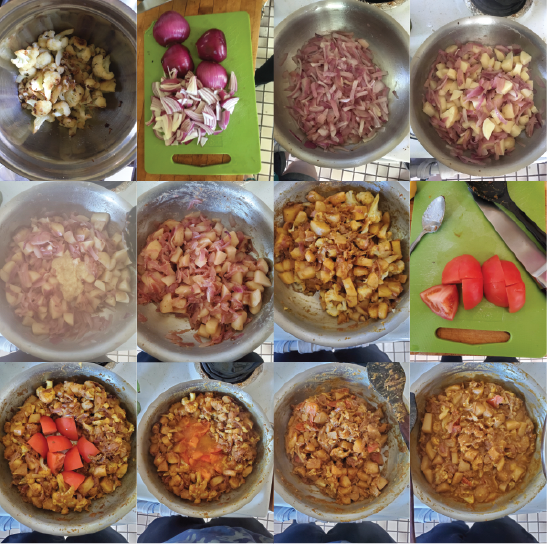
\includegraphics[width=1\textwidth]{recetas/Aloo-gobi/aloo-gobi.png}
\caption{Progresi\'on de la receta}
\label{fig:aloo-gobi}
\end{figure}

\end{enumerate}

\section{Italianas}
\subsection{Pizza Romano}

\textbf{Ingredientes (3 pizzas de 33 cm)}
\begin{itemize}
\item 3gr de levadura seca activa
\item 75gr de agua tibia
\item 225gr de harina de trigo
\item 225gr de harina de trigo entero
\item 225gr de agua fr\'ia
\item 9gr de sal
\item 200 gr de queso provolone dulce
\end{itemize}

\vspace{1cm}
\textbf{Instrucciones para masa}
\begin{enumerate}
\item Revolver la levadura en el agua caliente y dejarla por 10min
\item Revolver ésta \'ultima con la harina
\item Agregar el agua fr\'ia y revolver
\item Agregar la sal y amasar.
\item Poner en molde, con un fina capa de agua y cubrir. Dejar reposar por un día.
\end{enumerate} 


\subsection{Pizza Napolitana}


\textbf{Ingredientes (2 pizzas de 33 cm)}
\begin{itemize}
\item 6gr de levadura seca activa ($\sim$2 cucharaditas)
\item 75gr de agua tibia
\item 450gr de harina de trigo
\item 225gr de agua fr\'ia
\item 5gr de aceite de oliva ($\sim$1 cucharaditas)
\item 9gr de sal ($\sim$2 cucharaditas)
\item 1 bola de queso mozzarella (cortar en rodajas y dejar secar en estame\~na)
\item Albahaca

\end{itemize}

\subsection{Pasta fresca}
\textbf{Ingredientes}
\begin{itemize}
\item 200 gr de harina
\item 2 huevos
\item Sal al gusto ($\sim \sfrac{1}{2}$ cucharada)
\end{itemize}

\textbf{Instrucciones}
\begin{enumerate}
\item Mezclar todo y amasar hasta que este consistente ($\sim$10 min)
\item Envolver en plastico o toalla humeda y dejar reposar por media hora.
\item Extender en una superficie harinada lo m\'as que se pueda ($<$0.5 mm)
\item Cortar en la forma deseada (harinar si se va a guardar).
\item Cocer en agua hiriviendo por 3min.
\end{enumerate}

\subsection{Gnocchi di patate}
\textbf{Ingredientes}
\begin{itemize}
\item 150gr de harina
\item 500gr de papa
\item 30gr de huevo (medio huevo)
\end{itemize}

\textbf{Intrucciones}
\begin{enumerate}
\item Poner las papas en agua y apagar cuando empiece a hervir.
\item Pelar las papas
\item Rayar las papas o molerlas con un procesador.
\item Mezclar todo y amasar hasta que despegue ($\sim $20 min)
\item En una superficie harinada rodar y hacer rollitos de unos dos centimetros.
\item Cortar para que queden bolitas alargadas.
\item Rodar con un tenedor o una tablita dentada.
\item Dejar reposar por 15min.
\item Poner en agua hirviendo y sacar cuando floten ($\sim$1min)
\end{enumerate}


\section{Arroz}
\subsection{Arroz blanco simple}
\underline{Ingredientes}
\begin{itemize}
\item 1 taza de arroz
\item 1$\sfrac{1}{2}$ tazas de agua
\end{itemize}

\underline{Instrucciones}
\begin{enumerate}
\item En un sartén grande agregar el arroz y el agua.
\item Cocinar a fuego alto hasta que hierva.
\item Bajar al fuego MUY bajo y tapar.
\item Apagar cuando no quede agua.
\end{enumerate}


\subsection{Arroz a la mexicana}
\textbf{Ingredientes}
\begin{itemize}
\item 2 tomates medianos ($\sim$400gr)
\item 2 cucharaditas de aceite
\item 1 taza de arroz
\item 2 tazas de agua
\item Cubo de caldo de pollo (11gr)
\item Cuarto de cebolla ($\sim$ 70gr)
\item \sfrac{3}{4} de cucharadita de sal (o al gusto)
\item \sfrac{3}{4} de cucharadita de ajo en polvo (o al gusto)
\item Verdura cocida picada al gusto (zanahoria, elote o chicharo)
\end{itemize}

\textbf{Instrucciones}
\begin{enumerate}
\item Se hierven los tomates hasta que la cáscara se abra ($\sim$ 10min), se pelan y muelen.
\item \textit{Opcional}: Se lava el arroz hasta que el agua salga relativamente clara ($\sim$ 3 veces).
\item Se pone a hervir las dos tazas de agua y se disuelve el cubo de pollo.
\item Se precaliente un sartén con el aceite y se añade el arroz. Se mantiene en movimiento hasta que el arroz este amarillo. Se agrega la cebolla picada y se continua moviendo hasta que tenda un color dorado sin quemarse.
\item Se agrega y revuelve en el sart\'en el tomate, la sal, el ajo y el agua con el cubo de pollo.
\item Se deja a fuego lento, hasta que toda el agua se haya evaporado pero antes de que se pegue el arroz. Agregar las verduras un poco antes de esto si se desea.
\end{enumerate}

\subsection{Arroz verde}
\textbf{Ingredientes}
\begin{itemize}
\item 2 chiles poblanos ($\sim$250gr)
\item $\sim$ 20 ramas de cilantro (o al gusto)
\item 2 cucharaditas de aceite
\item 1 taza de arroz corto
\item 2\sfrac{1}{2} tazas de agua
\item Cubo de caldo de pollo (11gr)
\item Cuarto de cebolla ($\sim$ 70gr)
\item \sfrac{1}{2} de cucharadita de sal (o al gusto)
\item \sfrac{1}{2} de cucharadita de ajo en polvo (o al gusto)
\item Verdura cocida picada al gusto (zanahoria, elote o chicharo)
\end{itemize}

\textbf{Instrucciones}
\begin{enumerate}
\item Se ponen los chiles a fuego directo hasta que estan casi totalmente quemados homogeneamente. Se envuelven en plastico y se dejan reposar por 10min. Se pelan y remueven semillas y venas.
\item \textit{Opcional}: Se lava el arroz hasta que el agua salga relativamente clara ($\sim$ 3 veces).
\item Se pone a hervir el agua y se disuelve el cubo de pollo. Se licua junto con los chiles, el cilantro, el ajo y la sal.
\item Se precaliente un sartén con el aceite y se añade el arroz. Se mantiene en movimiento hasta que el arroz este amarillo. Se agrega la cebolla picada y se continua moviendo hasta que tenda un color dorado sin quemarse.
\item Se agrega y revuelve en el sart\'en la mezcla licuada.
\item Se deja a fuego lento, hasta que toda el agua se haya evaporado pero antes de que se pegue el arroz. Agregar las verduras un poco antes de esto si se desea.
\end{enumerate}

\subsection{Arroz para sushi}

\underline{Ingredientes}
\begin{itemize}
\item 1$\sfrac{1}{2}$ tazas de arroz medio/largo
\item 2 tazas de agua
\item $\sfrac{1}{4}$ de taza de vinagre
\item $\sfrac{1}{4}$ de taza de az\'ucar
\item $\sfrac{1}{2}$  cucharadita de sal
\end{itemize}

\underline{Instrucciones}

\begin{enumerate}
\item Lavar el arroz hasta que al agua salga clara ($\sim$5-7 veces) y escurrir.
\item Agregar el agua y cocinar a fuego alto hasta que comience a hervir.
\item Cocinar a fuego lento hasta que se evapore toda el agua.
\item Mezclar el vinagre, azucal y sal. Revolver la mezcla con el arroz y extender.
\item Utilizar hasta que se enfr\'ie.
\end{enumerate}


\section{Botana}
\subsection{Tzatziki}
\underline{Ingredientes}
\begin{itemize}
\item 250gr de yogurt griego (e.g. Fage)
\item $\sfrac{1}{2}$ pepino grande
\item 2 dientes de ajo finamente picados
\item $\sfrac{1}{2}$ cucharada de eneldo (\textit{dill}) finamente picado.
\item 1 cucharada de vinagre rojo/tinto
\item 2 cucharadas de aceite de oliva
\item $\sfrac{1}{4}$ de cucharadita de sal
\end{itemize}

\underline{Instrucciones}
\begin{enumerate}
\item Pelar el pepino y partirlo finamente. Si se tiene tiempo dejar secar para mejorar consistencia.
\item Revolcer el resto. Si se tiene tiempo dejar reposas en el refrigerador por unas horas.
\end{enumerate}


\section{Asi\'aticas}
\subsection{Estofado (receta de Elim)}
\underline{Ingredientes}
\begin{itemize}
\item 500gr de pollo/puerco/res/tofu en cuadritos
\item 2 papas medianas
\item 2 zanahorias
\item 1paguete con especias (\textit{spice pounch}. e.g. Tomax: anis, comino, clavo, regaliz, canela, nuez moscada y laurel)
\item 4 dientes de ajo finamente picados
\item 4 cucharadas de aceite de sesamo
\item 2 cebollines rebanados
\item 4 rebanadas de gengibre finamente picadas
\item 2 cucharada de pasta koreana (\textit{Doenjang, korean bean past}. e.g. Chung Jung One Sunchang Ssamjang)
\item 4 cucharadas de vino de cocinar japon\'es (\textit{mirin})
\item 4 cucharadas de salsa de soya
\item Chile seco al gusto (1-2 cucharadas) (red chilli pepper flakes)
\end{itemize}

\underline{Instrucciones}
\begin{enumerate}
\item Pelar y cortar en trozos peque\~nos (1-2 cm de lado) la papas y la zanahoria
\item Hacer una salsa mezclando la pasta koreana, el vino, la salsa de soya y el chile seco.
\item En un sartén grande calentar 2 cucharadas de aceite y echar el ajo y el gengibre.
\item Apenas desprenda olor, antes de que se queme, agregar la papa, la zanahoria, la salsa, el paquete de especias y agua hasta que se cubra.
\item Deja a fuego alto hasta que se evapore el agua y se obtenga una consistencia espesa. Remover el pequete de especias.
\item Freir la carne o tofu con dos cucharadas de aceite de sesamo.
\item Mezclar todo y poner los cebollines arriba.
\item Acompañar con arroz blanco simple
\end{enumerate}


\section{Pollo}
\subsection{Coachala}

{\color{red} En desarrollo}

Fuente: recetario mamá\\

\underline{Ingredientes}

\begin{itemize}
\item 1 gallina grande \footnote{Quizá para un pollo de 1.5kg sea suficiente con la mitad de los ingredientes. Actualizar.}
\item 1 kilo de masa
\item 200 gr de chile ancho
\item 200 gr de manteca
\item \sfrac{1}{2} kg de tomate verde
\item 1 cabeza de ajo
\item Sal al gusto
\end{itemize}

\underline{Instrucciones}

\begin{enumerate}
\item Cocer la gallina (\Sim 20 en olla a presión)
\item Desmunzar pechuga, hígado, corazón y mollejas
\item Licuar el resto de la carne con el caldo en el que se coció.
\item Dorar los chiles ligeramente, sin semilla.
\item Cocer lo tomates hasta que revienten
\item Licuar los tomates, el ajo, los chiles y caldo.
\item Colar la salsa
\item Añadir agua a la masa para hacer un atole espeso y llevar a hervor.
\item Mezclar todo y llevar a hervor, meneando todo el tiempo.
\item Requemar la manteca y añadirla.
\item Añadir sal al gusto.
\item Dejar hervir, meneando, hasta que adquiera la consistencia adecuada.
\item Servir con tostadas, cebolla fresca y limón.
\end{enumerate}

\section{Mariscos}
\subsection{Camarones a la diabla}

Fuente: \href{https://www.youtube.com/watch?v=gDJC0GQnj7A}{Vicky Receta Fácil - Camarones a la diabla}
\\
\underline{Ingredientes}
\begin{itemize}
\item \sfrac{1}{2} kg de camarones
\item 3 dientes de ajo
\item 2 limones
\item 2 jitomates
\item \sfrac{1}{8} de cebolla
\item 3 chiles guajillos sin semilla
\item Chiles de árbol la gusto
\item 1 chile chipotle de lata
\item 1 cubo de caldo de pollo
\item 2 cucharadas de matequilla
\item 1 cuchara de aceite de oliva
\item Sal al gusto
\item Pimienta al gusto
\end{itemize}

\underline{Instrucciones}

\begin{enumerate}
\item Cocer los tomates, los chiles de árbol y guajillo.
\item Licuar los chiles con la cebolla, un diente de ajo, el limon, el caldo de pollo y un poco de agua.
\item Colar la salsa
\item Derretir la mantequilla a fuego bajo
\item Añadir el aceite
\item Agregar dos ajos triturados y cocer por unos segundos
\item Agregar los camarones y cocer mezclando a fuego bajo hasta que estén rosas.
\item Agregar pimienta y sal
\item Agregar la salsa y dejar hervir por 1min.
\end{enumerate}

\section{Pan}
\subsection{Pan de caja}

\underline{Ingredientes}

\begin{itemize}
\item 250 gr de harina
\item 250 gr de harina integral
\item 2 cucharadita de sal
\item 2 cucharadita de levadura
\item 380gr de agua
\item Aceite de oliva (para engrasar)
\end{itemize}

\underline{Instrucciones}

\begin{enumerate}
\item Mezclar la levadura en 80ml de agua tibia.
\item Mezclar con el resto de los ingredientes y amasar.
\item Dejar reposar por \Sim1.5hrs (hasta que doble el tamaño).
\item Poner en un molde de panque engrasado con aceite y esperar 1-2hrs a que duplique su tamaño.
\item Hornear por \Sim35min a 200C (400F).
\end{enumerate}

\subsection{Baguettes con poolish}

Fuente: How to make bread por Emmanuel Hadjiandreou

\underline{Ingredientes}
\textbf{Ingredientes para el prefermento}
\begin{itemize}
\item $\sfrac{1}{4}$ de cucharadita de levadura (2g)
\item 125 ml de agua tibia
\item 125 gr de harina
\end{itemize}

\textbf{Ingredientes para el resto}
\begin{itemize}
\item $\sfrac{1}{4}$ de cucharadita de levadura (2g)
\item 300 gr de harina
\item 5 gr de sal
\item 140 ml de agua tibia
\end{itemize}

\underline{Instrucciones}
\begin{enumerate}
\item Preparar el pre-fermento
\begin{itemize}
\item Diluir la levadura en el agua tibia
\item Mezclar la harina
\item Dejar reposar cubierta en plástico durante la noche.
\end{itemize} 
\item Mezclar la sal con la harina
\item Diluir la levadura en el agua tibia.
\item El agua con la harina y amasar hasta que esta lisa. Puedes trabajar en una superficie enharinada, pero cuidando de no usar mucha.
\item Dejar reposar en un molde cubierto con plástico por \Sim 1hr (hasta que doble su tamaño).
\item Dividir en 3. Cada pedazo se alarga en una superficie con harina, doblandose sobre si mismo, hasta que tenga \Sim 30 cm de largo.
\item Dejar reposar en dobleces de una manta para pan (couche / proofing linen), con el dobles hacia arriba, por \Sim 1hr (hasta que doble su tamaño.)
\item Pasar a una pala con el dobles hacia abajo.
\item Hace cortes superficiales con una navaja de afeitar.
\item Pasar a la piedra en el horno, precalentado a 240 C (475 F), y hornear a 10-15 min. Rociar agua a las parades del horno durante los primeros 6 min, cada 1-2 min\footnote{De forma alternativa puedes calentar un sarten de hierro fundido, ponerlo en el fondo y vaciar agua.}.
\end{enumerate}


\section{Quesos}
\subsection{Queso panela}

Basada en : \href{http://www.sagarpa.gob.mx/desarrolloRural/Documents/fichasaapt/Elaboraci%C3%B3n%20de%20quesos.pdf}{SAGARPA - Elaboración de quesos tipo Panela y Oaxaca} \\

\underline{Ingredientes}
\begin{itemize}
\item 4 litros de leche pasteurizada \footnote{De preferencia pasteurizada a bajas temperaturas y no homogeneizada. Quitar crema si no está homogeneizada. No usar leche ultra-pasteurizada.}
\item $\sfrac{1}{4}$ de pastilla para cuajar \footnote{Puede variar dependiendo de la marca. Usé Walcoren que cuajaba hasta 
\Sim 20litros por pastilla.}
\item 30-40gr de sal
\item 1 cucharadita de cloruro de calcio al 32\% en peso \footnote{Opcional. Mejora el rendimiento}
\end{itemize}


\underline{Instrucciones}
\begin{enumerate}
\item Calentar la leche a \Sim 32 C
\item Disolver la pastilla para cuajar en un poco de agua y revolver en la leche.
\item Dejar reposar hasta que cuaje y se pueda cortar (30-60 min).
\item Hacer varios cortes especiados por un par de centimetros, en ambas direcciones.
\item Calentar muy lentamente hasta \Sim 32 C mientras se menea para separar el suero.
\item Dejar reposar por 15 min.
\item Con la ayuda de un colador remover el suero \footnote{Has queso ricotta (\ref{queso-ricotta}) con el suero.}, pero sin exprimir.
\item Revolver la cuajada con la sal. Usar 3\% del peso del cuajo.
\item Poner en un molde con estame\~na y exprimir suavemente el suero excedente.
\item Dejar reposar durante 15 min, voltear, y dejar reposar por 3 horas.
\end{enumerate}

\subsection{Queso ricotta}\label{queso-ricotta}

Basada en : \href{https://www.culturesforhealth.com/learn/recipe/cheese-recipes/whey-traditional-ricotta-cheese/}{Cultures for health - Traditional whey ricotta} \\

\underline{Ingredientes}
\begin{itemize}
\item 2 lt de suero de leche
\item 2 cucharadas de jugo limon o vinagre
\item Sal al gusto
\end{itemize}


\underline{Instrucciones}
\begin{enumerate}
\item Calentar el suero sin que llegue a hervir (\Sim 195F o 90C).
\item Agregar el jugo de limon o vinagre y revolver.
\item Esperar 15 min.
\item Vaciar en un colador o estame\~na. Dejar escurrir for varias horas.
\item Agregar sal al gusto.
\end{enumerate}

\subsection{Paneer}

Basada en : \href{http://www.madhurasrecipe.com/veg/Homemade-Paneer}{Homemade paneer - Madhura's recipe} \\

\underline{Ingredientes}
\begin{itemize}
\item 1 gal\'on (3.8L) de leche pasteurizada \footnote{De preferencia pasteurizada a bajas temperaturas y no homogeneizada. Quitar crema si no está homogeneizada. No usar leche ultra-pasteurizada.}
\item $\sfrac{1}{2}$ taza de jugo de limon
\end{itemize}


\underline{Instrucciones}
\begin{enumerate}
\item Calentar la leche a punto de ebullición y apagar.
\item Agregar el limón y esperar unos minutos a que cuaje.
\item Poner en un molde con estame\~na y exprimir suavemente el suero excedente \footnote{Quedó muy aguada, quizá debí de exprimir más?}.
\item Dejar reposar por ~30 min.
\end{enumerate}


\section{Postres}
\subsection{Yule log}

\underline{Ingredientes}

\textbf{Esponja}

\begin{itemize}
\item $\frac{1}{4}$ de taza de harina
\item 2 cucharadas de maicena
\item 2 cucharadas de cocoa
\item $\frac{1}{8}$ de cucharadita de sal
\item $\frac{1}{2}$ taza de az\'ucar
\item 2 huevos enteros
\item 3 yemas de huevo
\item 2 claras de huevo
\item 1 cucharadita de vainilla
\item $\frac{1}{4}$ de cucharadita de crema tartara
\item Un poco de azucar glass
\end{itemize}

\textbf{Relleno}

\begin{itemize}
\item 1 taza de heavy whipping cream
\item $\frac{1}{2}$ cucharadita de vainilla
\item $\frac{1}{4}$ de taza de azucar
\item 2 cucharadas de cocoa
\end{itemize}

\textbf{Ganache}

\begin{itemize}
\item 6 oz de chocolate oscuro
\item 2 oz de chocolate dulce (mil chocolate)
\item $\frac{3}{4}$ de taza de heavy whipping cream (fría)
\item 25 gr de mantequilla
\end{itemize}

\underline{Instrucciones}

\textbf{Esponja}

\begin{enumerate}
\item Cubrir de mantequilla un bandeja, poner un papel encerado, luego otra capa de mantequilla y enharinar.
\item Batir a alta velocidad los huevos enteros, las yemas, la vainilla y la azúcar menos una cucharada (guardar) por \Sim 3 min hasta que este espesa.
\item Añadir la harinna, la maicena, la sal y la cocoa de forma suave para no dejar escapar el aire.
\item Batir la crema tartara y las claras por unos segundos. Añadir la cucharada de azucar y batir a punto de turron.
\item Añadir este ultimo batido a la mezcla de forma suave.
\item Esparcir de forma uniforme en la bandeja.
\item Hornear a 450 F (230 C) por 6 min. Que este bien cocido pero evitar que se seque y endurezca.
\item Espolvorear la azucar glass sobre la esponja.
\item Volvear sobre una toalla
\item Espolvorear azucar glass sobre el otro lado
\item Enrollar y dejar que se enfrie
\end{enumerate}

\textbf{Ganache}

\begin{enumerate}
\item Calentar la whipping cream y la mantequilla hasta que comienze a hervir y sacar de la estufa.
\item Añadir el chocolate y mezclar hasta que se derrita y este uniforme.
\item Dejar reposar hasta que se enfríe y este untable. Si se mete el refri para acelerar el procesos menear cada 10 min.
\end{enumerate}

\textbf{Relleno}
\begin{enumerate}
\item Batir todo hasta que este bien firme
\end{enumerate}

\textbf{Final}
\begin{itemize}
\item Desenrollar la esponja
\item Untar el relleno de forma uniforme por dentro
\item Enrollar
\item Cubrir con el ganache
\end{itemize}


\subsection{Capirotada}
\underline{Ingredientes}
\begin{itemize}
\item 1 jitomate pequeño picado ($\sim$150gr)
\item $\sfrac{1}{4}$ de cebolla pequeña picada ($\sim$50gr)
\item 1 litro de agua
\item 250 gr de piloncillo (panocha, panela)
\item 4 clavos de olor
\item 2 rajas de canela
\item 250 gr de pan seco \footnote{o secar por 30min en el horno a 150$^\circ $C (300$^\circ $F)}
\item 1 platano o al gusto (de preferencia macho)
\item 1 taza de cacahuates o al gusto
\item $\sfrac{1}{2}$ taza de pasitas o al gusto
\end{itemize}

\underline{Instrucciones}

\begin{enumerate}
\item Poner a hervir el agua con los jitomates, piloncillo, cebolla, clavos y canela por 15min.
\item Colar todos los s\'olidos
\item En un refractario colocar una capa de pan, pasitas, platano, cacahuates y agua de piloncillo. Aplastar ligeramente para que quede homogenea y continuar hasta acabarse todo (2-3 capas).
\item Hornear a 180$^\circ $C (35$^\circ $F) por 25min.
\item Servir fr\'ia.
\end{enumerate}

\subsection{Pastel de zanahoria y bet\'un}

\underline{Ingredientes}
\begin{itemize}
\item 1 taza de harina
\item 1 taza de azucar
\item $\sfrac{1}{2}$ cucharadita de bicarbonato
\item $\sfrac{1}{2}$ cucharadita de levadura qu\'imica
\item $\sfrac{1}{4}$ de cucharadita de sal
\item $\sfrac{3}{4}$ de taza de aceite vegetal
\item 2 huevos
\item 1$\sfrac{1}{2}$ tazas de zanahoria rallada
\item $\sfrac{1}{4}$ de taza de nuez molida
\item 1 cucharadita de vainilla
\item $\sfrac{1}{2}$ cucharadita de canela molida
\item $\sfrac{1}{4}$ de taza de pasitas
\end{itemize}

\underline{Instrucciones}
\begin{enumerate}
\item Hacer una mezcla homogenea y hornear a 180$^\circ$ (350$^\circ$F) hasta tan pronto como este firme ($\sim$20-30 min para cupcakes, $~$50-60 min en un molde grande).\\
\end{enumerate}

\textbf{Betún}

\underline{Ingredientes}
\begin{itemize}
\item 1 paquete de queso Philadelphia (8 oz)
\item 1 barra de mantequilla (4 oz)
\item 6 tazas de azucar glass
\end{itemize}

\underline{Instrucciones}
\begin{enumerate}
\item Batir la mantequilla hasta que este cremosa.
\item Agregar el queso y batir hasta que no haya grumos.
\item Mezclar con la az\'ucar un poco a la vez, hasta que este homog\'eneo
\item Refrigerar un tiempo para mejorar consistencia.
\end{enumerate}


\subsection{Pan de calabaza}

\underline{Ingredientes}\\
Para molde redondo, duplicar para molde de panqué
\begin{itemize}
\item 1 taza de harina
\item $\sfrac{1}{2}+\sfrac{1}{3}$ tazas de azucar
\item $\sfrac{1}{2}$ cucharadita de bicarbonato
\item $1$ cucharadita de levadura qu\'imica
\item $\sfrac{1}{2}$ de cucharadita de sal
\item $\sfrac{1}{2}$ de taza de aceite vegetal
\item 2 huevos
\item 7.5 oz de pulpa de calabaza
\item $1$ cucharadita de canela molida
\item Harina y mantequilla para el molde
\end{itemize}

\underline{Instrucciones pulpa de calabaza}
\begin{enumerate}
\item Limpiar la calabaza y cortarla en gajos
\item Poner en el horno a 200$^\circ$ (400$^\circ$F) por una hora o hasta que este blanda.
\item Quitar c\'ascara y moler en procesador.
\end{enumerate}

\underline{Instrucciones}
\begin{enumerate}
\item Hacer una mezcla homogenea.
\item Cocinar en el horno a 180$^\circ$ (350$^\circ$F) por 20 min en molde redondo o \Sim80 min en molde de panqu\'e (hasta que est\'e s\'olido, sin secarse)\\
\end{enumerate}

\subsection{Muffins de banana}

\underline{Ingredientes}
\begin{itemize}
\item \sfrac{1}{4} de taza de leche
\item 1 cucharada vinagre
\item 3 pl\'atanos
\item 1 taza de azucar
\item 2 huevos
\item \sfrac{3}{4} de taza de aceite vegetal
\item 2 tazas de harina
\item 2 cucharaditas de bicarbonato de sodio
\end{itemize}

\underline{Instrucciones}
\begin{enumerate}
\item Mezclar la leche con el vinagre y deja reposar por 10 min.
\item Mezclar el resto de los ingredientes en el orden en el que aparecen
\item Hechar tres cucharadas de la mezcla de leche y vinagre en la mezcla principal, y mezclar.
\item Hornear a 180$^\circ$C (350$^\circ$F) hasta que este firme ($\sim$20-30min).
\end{enumerate}

\subsection{Dulce de calabaza}

\underline{Ingredientes}
\begin{itemize}
\item Calabaza
\item Cal
\item Azucar
\item Vainilla
\end{itemize}

\underline{Instrucciones}
\begin{enumerate}
\item Cortar la calabaza en trozos peque\~nos
\item Se deja remojar la calabaza por 24 horas en una mezcla de agua y cal en proporci\'on 1 litro : 1 cucharada.
\item Enjuagar la calabaza.
\item Poner a cocer la calabaza a fuego lento en un mezcla de agua, azucar y vainilla en una proporcion de 1 litro : 1 kg : 1.5 cucharadas.
\item Remover cuando la mayor parte del agua se haya evaporado y s\'olo quede melcocha. 
\end{enumerate}

\subsection{Conchas}

\underline{Ingredientes}\\
\textbf{Masa}
\begin{itemize}
\item 250 gr de harina
\item 5 gr de sal (\Sim 1 cucharadita)
\item 7 gr de levadura (\Sim 2 $\sfrac{1}{2}$ cucharaditas)
\item 2 huevos +  barniz
\item 50 gr de mantequilla sin sal (a temperatura ambiente)
\item 50 ml de agua tibia
\item 50 ml de agua fria
\item 40 gr de azucar
\end{itemize}


\textbf{Tapa blanca}
\begin{itemize}
\item 100 gr de manteca vegetal
\item 100 gr de azucar glass
\item 100 gr de harina
\end{itemize}

\textbf{Tapa de chocolate}
\begin{itemize}
\item 100 gr de manteca vegetal
\item 100 gr de azucar glass
\item 16 gr de cocoa
\item 84 gr de harina
\end{itemize}

\underline{Preparaci\'on}

\begin{enumerate}
\item Mezclar la levadura con el agua tibia para activarla
\item Amasar todo hasta que despegue, estirando y con ayuda de una espátula (a mano toma $\sim$1 hora, en KitchenAid $\sim$10 min)
\item Dejar fermentar hasta que doble el tamaño
\item Hacer bolas de 50gr.
\item Barnizar con huevo (capa muy delgada).
\item Hacer la mezcla de las tapas
\item Hacer las tapas (25gr) con ayuda de harina para que no se pegue. 
\item Acomodar tapa y marcar (enharinar el marcador).
\item Hornear a 200C (400F) por 12min.
\end{enumerate}

\subsection{Jericalla}
\underline{Ingredientes}
\begin{itemize}
\item 2 tazas de leche
\item 2 huevos 
\item $\sfrac{1}{2}$ taza de azucar
\item 2 cucharadas de vainilla
\item 1 raja de canela
\end{itemize}

\underline{Preparaci\'on}
\begin{enumerate}
\item Poner a hervir todo excepto el huevo por 10 min, agitando continuamente.
\item Esperar a que se enfr\'ie.
\item Revolver con el huevo.
\item Poner a hornear a ba\~no mar\'ia en moldes peque\~nos a 205°C (400°F) hasta que tenga manchas negras en la cubierta ($\sim$1.5 horas). 
\end{enumerate}

\subsection{Flan napolitano}
\underline{Ingredientes}
\begin{itemize}
\item \sfrac{1}{2} de taza de az\'ucar
\item 4 huevos
\item 1 lata de leche condensada (397 gr)
\item 1 taza de leche evaporada
\item 1 cucharadita de vainilla
\item 10 oz de queso crema
\end{itemize}

\underline{Preparaci\'on}
\begin{enumerate}
\item Calentar el azucar a fuego lento y meneando. Apagar tan pronto como toda este derretida.
\item Verter la azucar derretida en el fondo de una flanera y dejar que llegue a temperatura ambiente.
\item Licuar el resto de los ingredientes y verter en la flanera.
\item Hornear en baño mar\'ia a 200$^\circ$C (400F) por 1hr.
\item Sacar del horno y esperar a que llegue a temperatura ambiente. Luego refrigerar por varias horas hasta que tenga la temperatura de equilibrio.
\item Servir volteado.
\end{enumerate}

\subsection{Pay de queso}
\underline{Ingredientes}
\begin{itemize}
\item Un paquete de galletas mar\'ia (170gr)
\item Una barra de matequilla (113gr) + engrasar molde
\item Un paquete de queso crema (8oz)
\item 2 huevos
\item 1 cucharadita de vainilla
\item \sfrac{1}{2} lata de leche condensada (200gr)
\item \sfrac{1}{2} lata de leche evaporada (170gr)
\end{itemize}

\underline{Preparai\'on}
\begin{itemize}
\item Dejar que la mantequilla este a temperatura ambiente
\item Hacer polvo las galletas mar\'ia.
\item Hacer una masa homogenea con el polvo de galletas y la mantequilla
\item Engrasar el molde con una capa de mantequilla.
\item Poner una capa homogenea de la masa de galletas y mantequilla en todo el molde.
\item Licuar el resto de los ingredientes y verter en el molde
\item Hornear por 45 min a 180C (350F).
\item Sacar y dejar que llegue a temperatura ambiente. Despues meter el refrigerador y dejar que llegue a la temperatura interna de este. 
\end{itemize}

\subsection{Galletas de mantequilla}
\underline{Ingredientes}
\begin{itemize}
\item 150 gr de mantequilla
\item 125 gr de azucar
\item 1 huevo
\item 175 gr de harina
\item 1 cucharadita de canela molida
\item Pizca de sal
\end{itemize}

\underline{Instrucciones}
\begin{enumerate}
\item Dejar la mantequilla afuera del refrigerador hasta que se suavice. 
\item Mezclar la mantequilla con el az\'ucar hasta que este cremoso.
\item Agregar el huevo y mezclar.
\item Agregar el resto y mezclar.
\item Meter la mezcla cubierta con plastico al refrigerador por $\sim$20 min.
\item En una superficie harinada extender la masa hasta que tenga 5-7mm de espesor.
\item Cortar de la forma deseada y poner en un charola con papel encerado (o con mantequilla+harina).
\item Volver a hacer bola el sobrante de masa y repetir.
\item Hornear por $\sim$20 min a 180$^\circ$C hasta que las orillas esten cafes.
\end{enumerate}

\subsection{Rosca de Reyes}

Basada en : \href{https://www.youtube.com/watch?v=4IgNDiX7cHg}{Vicky Receta Facil - Rosca de Reyes}. Yo uso un huevo extra.\\

\underline{Ingredientes}

\textbf{Masa}
\begin{itemize}
\item 135 gr de mantequilla
\item 4 huevos
\item \sfrac{1}{2} taza de leche tibia
\item \sfrac{3}{4} de taza de azucar
\item 1 cucharadita de sal
\item 11 gr de levadura
\item 2 cucharaditas de vainilla
\item \sfrac{1}{2} kg de harina
\end{itemize}

\textbf{Costra}
\begin{itemize}
\item 100 gr de manteca vegetal
\item 100 gr de harina
\item 100 gr de azucar glass
\item 2 yemas de huevo
\end{itemize}

\textbf{Extras}
\begin{itemize}
\item Ate (e.g. mebrillo, guayaba, tecojote)
\item Higos cristalizados
\item Cerezas en almibar
\item Azucar
\item 1 huevo
\item Monitos
\end{itemize}

\underline{Instrucciones}
\begin{enumerate}
\item Poner la levadura en leche tibia, con una cucharada de azucar y una de harina. Dejar deposar hasta que las burbujas dupliquen el tamaño.
\item Amasar el resto de los ingrediente de la masa hasta que despegue.
\item Dejar reposar cubiertas hasta que duplique su tamaño (\Sim 1.5 hr).
\item En una superficie harinada hacer una tira de 1m de largo.
\item Meter monitos por abajo.
\item Hacer la rosca en una charola engrasada. Las puntas se unen haciendo un hueco de un lado y un pico del otro.
\item Mezclar lo ingredientes de la costra hasta que este homogenea.
\item Barnizar con una capa delgada de huevo
\item Poner costa y dulces. Espolvorear azucar en la costra.
\item Dejarla reposar por 30 min.
\item Hornear a 180C (350F) por 20 min.
\end{enumerate}

\subsection{Pastel de tres leches}

Basada en: \href{https://www.elmejornido.com/es/recetas/pastel-tres-leches-121630}{Pastel de tres leches - El mejor nido}\\

\underline{Ingredientes}

\textbf{Pan (por piso, hacer 3 pisos)}

\begin{itemize}
\item 3 claras de huevo
\item 3 yemas de huevo
\item 4 cucharadas de az\'ucar (uso dividido)
\item $\sfrac{1}{2}$ taza de harina 
\end{itemize}

\textbf{Jugo}

\begin{itemize}
\item 1 lata (14oz) de leche condensada
\item 1 lata (7.6 fl. oz.) de media crema o 1 taza de whipping cream
\item $\sfrac{2}{3}$ de taza de leche evaporada
\item $\sfrac{1}{4}$ de taza de brandy\footnote{Probar con más, la última vez que lo hice no sabía mucho. Quizá fue por usar amaretto.}
\item 1 cucharadita de vainilla
\end{itemize}

\textbf{Crema batida}

\begin{itemize}
\item 1 taza de whipping cream
\item 2 cucharadas de azucar
\item $\frac{1}{2}$ cucharadita de vainilla
\end{itemize}

\textbf{Extras}
\begin{itemize}
\item Mermelada (entre las capas)
\item Mantequilla y harina (para el molde)
\end{itemize}

\underline{Instrucciones}

\textbf{Pan}
\begin{enumerate}
\item Batir las claras y 2 cucharadas de az\'ucar a punto de turrón
\item Batir las yemas y 2 cucharadas de az\'uzar hasta que este homog\'eneo
\item Incorporas los dos batidos y la harina con movimientos envolvientes suaves
\item Hornear a 375 F (190 C) en un molde engrasado y enharinado hasta que pase la prueba dle palillo (\Sim 12 min para un molde redondo de 9in).
\end{enumerate}

\textbf{Jugo}
\begin{enumerate}
\item Mezclar todo bien hasta que esté homogéneo
\end{enumerate}

\textbf{Crema batida}
\begin{enumerate}
\item Batir todo hasta que esté firme
\end{enumerate}

\textbf{Todo}
\begin{enumerate}
\item Poner una capa pan en donde se va a servir y con un tenedor o palillo agujerearla toda.
\item Ir mojando con el jugo poco a poco dejando que se absorba, hasta que ya no pueda absorver más\footnote{Me parece que es mejor hacerlo mientras el man esta caliente para que se sature más f\'acilmente.}.
\item Poner un capa de mermelada
\item Repetir con las otras dos capas.
\item Forrar con crema batida.
\end{enumerate}
\subsection{Chongos zamoranos}

\underline{Ingredientes}

\begin{itemize}
\item 1 litro de leche \footnote{Usar de preferencia leche bronca. Si se usa pasterurizada, de prefencia que haya sido pasteurizada a temperaturas bajas y que no esté homogeneizada. No usar leche ultra-pasteurizada.}
\item 1 taza de azucar morena
\item $\sfrac{1}{4}$ pastilla de cuajar \footnote{Usar pastillas para cuajar que se utilicen en la fabricación de queso. No usar "Junket". La cantidad puede variar dependiendo de la marca.}
\item 2 o 3 rajas canela
\end{itemize}

\underline{Instrucciones}
\begin{enumerate}
\item Disolver la pastilla en un poco de agua.
\item Calentar la leche hasta que esté tibia.
\item Agregar la pastilla disuelta a la leche y esperar a que cuaje (1-2 hrs). Esta lista cuando se puedar cortar con un cuchillo.
\item Cortar en \Sim 12 pedazos. El tamaño debe de ser mas o menos del sobre del tamaño final deseado.
\item Poner a fuego medio hasta que hierva
\item Insertar las rajas de canela y agregar el azúcar
\item Dejar hervir por dos horas a fuego muy bajo.
\end{enumerate}
\subsection{Galletas de doble chocolate}
\underline{Ingredientes}
\begin{itemize}
\item 1 taza de harina ($\sim$145 gr)
\item $\sfrac{1}{2}$ cdita de polvo para hornear
\item $\sfrac{1}{2}$ cdita de bicarbonato de sodio
\item $\sfrac{3}{4}$ cdita de sal kosher (grano poco mas grueso) 
\item $1\sfrac{1}{4}$ barras de mantequilla ($\sim$10 cdas. o $\sim$ 141 gr)
\item $\sfrac{3}{4}$ taza de cacao en polvo ($\sim$ 75 gr)
\item 1 huevo
\item 2 cditas de extracto vainilla
\item $\sfrac{1}{2}$ taza de az\'ucar morena 
\item $\sfrac{1}{2}$ taza de az\'ucar blanca 
\item 2 tazas de chispas o discos de chocolate semi-amargo ($\sim$ 315 gr)
\end{itemize}

\underline{Instrucciones}

\begin{enumerate}
\item Acremar mantequilla con az\'ucar. 
\item Incorporar huevo y vainilla.
\item Homogeneizar por separado el harina, el polvo para hornear, el bicarbonato, la sal y el polvo de cacao.
\item Incorporar los ingredientes secos a la mezcla con mantequilla.
\item Agregar las chispas/discos de chocolate y cubrir la masa con pl\'astico, luego enfriar al menos 24 horas, pero no mas de 36.
\item Hacer bolitas de 3 $\sfrac{1}{2}$ oz (un poco mas grandes que una pelota de golf) y espaciarlas bien ya que se extienden bastante al hornear. 
\item Hornear a 180$^\circ $C (35$^\circ $F) por 18 min. Enfriar en un rack.
\item Servir tibias.
\end{enumerate}

\subsection{Torta de calabacita}

Basada en: recetario abuelita \\

\underline{Ingredientes}
\begin{itemize}
\item $\sfrac{3}{4}$ kg de calabacita
\item $\sfrac{1}{4}$ kg de harina de arroz
\item 2 cucharaditas de polvo para hornear
\item 100 gr de mantequilla (temperatura ambiente)
\item 3 huevos
\item 100 gr de queso cotija
\item 1 taza de azúcar
\item Mantequilla y pan molido para el molde.
\end{itemize}

\underline{Instrucciones}
\begin{enumerate}
\item Poner a hervir agua con un poco de sal y cocer las calabacitas por 5 min.
\item Molerlas/licuarlas y dejar escurrir el agua sobrante.
\item Acremar la mantequilla con el azúcar. 
\item Batir con los huevos.
\item Añadir la calabacita molida, la harina arroz, el polvo para hornear y el queso, y mezclar.
\item Recubrir el molde con mantequilla y pan molido.
\item Hornear a 180C (350F) por \Sim 40min, hasta que pase la prueba dle palillo.
\end{enumerate}

\subsection{Chocolate Mousse Cake}

Fuente: \href{https://www.lifeloveandsugar.com/2017/10/23/chocolate-mousse-cake/}{Life, love and sugar - Chocolate Mousse Cake}\\

\underline{Ingredientes}

\textbf{Pan}
\begin{itemize}
\item 230gr de harina
\item 420 gr de azúcar
\item 85 gr de cocoa
\item 2 $\sfrac{1}{4}$ cucharaditas de bicarbonato de sodio
\item $\sfrac{1}{2}$ cucharaditas de polvo para hornear
\item 1 cucharadita de sal
\item 1 taza de leche
\item $\sfrac{1}{2}$ tazas de aceite vegetal
\item 1 $\sfrac{1}{2}$ cucharaditas de vainilla
\item 2 huevos
\item 1 taza de agua caliente
\item Mantequilla para el molde
\end{itemize}

\textbf{Mousse}
\begin{itemize}
\item 4 yemas de huevo
\item $\sfrac{1}{4}$ tazas de azúcar
\item 1 $\sfrac{3}{4}$ tazas de heavy whipping cream
\item 225gr de chocolate en barra
\item 85 gr de azúcar glass 
\end{itemize}

\textbf{Betun}
\begin{itemize}
\item 2 $\sfrac{1}{2}$ tazas de heavy whipping cream
\item 70 gr de azúcar glass
\item 60 gr de cocoa
\item 1 cucharadita de vainilla
\end{itemize}

\underline{Instrucciones}

\textbf{Pan}
\begin{enumerate}
\item Combinar ingredientes secos, luego líquidos, excepto el agua. Mezclar el agua al final.
\item Dividir en tres moldes redondos. Estos deben de tener matenquilla en el fondo y una capa de papel encerado.
\item Hornear a 350 F (180 C) por 20-25min, hasta que pase la prueba del palillo.
\end{enumerate}

\textbf{Mousse}
\begin{enumerate}
\item Mezclar las yemas, el azúcar y media taza de whipping cream. Cocinar a baño maría por \Sim 10min mezclando continuamente hasta que espese y adquiera volumen. El agua debe de mantenerse a \Sim 70C.
\item Derretir el chocolate a baño maría.
\item Añadir a la primera mezcla y batir hasta que esté suave.  Dejar enfríar.
\item Batir el resto de la whipping cream (1$\sfrac{1}{4}$ de taza) con la azúcar glass hasta que forme picos.
\item Mezclar todo con movimiento envolventes, agregando de a poco a la vez.
\end{enumerate}

\textbf{Betún}
\begin{enumerate}
\item Bartir todo hasta que forme picos
\end{enumerate}

\textbf{General}
\begin{enumerate}
\item Hacer el pan y dejar enfriar.
\item Hacer el mousse.
\item Emparejar los panes con un chuchillo si es necesario.
\item Con la ayuda de un "cake collar" poner el mousse en medio de los panes. Dejar en el refrigerador por \Sim 5 horas.
\item Hacer el betún y cubrir. 
\item De preferencia dejar en el refrigerador una noche.
\end{enumerate}
\subsection{Besos de novia}

Basada en: \href{https://www.youtube.com/watch?v=V18ECzDqUjM}{BESOS DE NOVIA - Fernanda Berlei
} \\

También llamados polvorones, bolitas de nuez, pedos de monja o galletas de boda.

\underline{Ingredientes}

\begin{itemize}
\item 225 gr de mantequilla sin sal
\item Azúcar glass
\begin{itemize}
\item 90 gr para la masa
\item Extra para espolvorear
\end{itemize}
\item 300gr de harina de trigo
\item 1 $\sfrac{1}{2}$ cucharaditas de canela en polvo
\item Nuez molida
\begin{itemize}
\item 200gr bien molida (polvo).
\item Opcional: agregar pedacitos a la masa
\end{itemize}
\end{itemize}


\underline{Instrucciones}

\begin{enumerate}
\item Acremar la mantequilla
\item Agregar el azucar y mezclar
\item Agregar y mezclar la canela, harina y nueces
\item Hacer bolitas del approximadamente un cucharada y poner en una bandeja encerada o con papel encerado.
\item Hornear a 180 C (360F) hasta que la orilla este ligeramente dorada (15-20min).
\item Revolcar en azúcar glass.
\end{enumerate}


\subsection{Hojaldre}

Basada en: \href{https://elcomidista.elpais.com/elcomidista/2017/02/08/receta/1486577378_084473.html}{LA CIENCIA DE HACER HOJALDRE - El Comidista} y  \href{https://www.meilleurduchef.com/fr/recette/pate-feuilletee.html}{Pâte feuilletée - Meilleur du Chef}\\

\underline{Ingredientes}

\begin{itemize}
\item 500 gr de harina
\item 250 ml de agua
\item 10 gr de sal
\item 500 gr de mantequilla
\item Harina para espolvorear
\end{itemize}

\underline{Instrucciones}

\begin{enumerate}
\item Sacar la mantequilla del refri, o si esta afuera meterla un tiempo, tal que esté maleable pero no aguada.
\item Si la mantequilla no es un sólo bloque, amasar un poco para que todos los pedazos de integren.
\item Con ayuda de una bolsa o papel encerado, así como un rodillo y una espátula, aplanar la mantequilla hasta forme un cuadrado de \Sim 1cm de alto.
\item Mezclar la harina y la sal. Integrar el agua poco a poco.
\item Amasar un poco. La masa debe de estar homogénea pero no se necesita amasar mucho, no se necesita que esté lisa.
\item Envolver con plástico y dejar reposar por una hora a temperatura ambiente.
\item Envolver el bloque de mantequilla con la masa como se muestra en la Figura \ref{fig:envoltura-hojaldre}:
\begin{enumerate}
\item La masa de hace una bola y se hacen dos cortadas que vayan hasta mitad de la bola, tal que queden cuatro picos
\item Trabajar sobre una superfifie enharinada.
\item Los picos se extienden con un rodillo. 
\item Todo se extiende con el rodillo hasta que el cuadrado del centro tenga el tamaño de la mantequilla. Los extremos deben de tener el mismo tamaño que el centro pero más delgados.
\item Poner la mantequilla en el centro y envolver con los extremos. Cada vez que se dobla un extremo remover la harina con una brocha.
\item Cuidar que las orillas queden cerradas y cubiertas por la masa.
\end{enumerate}
\item Envolver con plástico y meter el refri durante la noche o al menos un par de horas, hasta que la masa endurezca.
\item Estirar y doblar como se muestra en la Figura \ref{fig:doblado-hojaldre} 6 veces:
\begin{itemize}
\item Si la masa esta muy dura, sobre todo la primera vez, dar uno golpecitos con el rodillo a lo largo y ancho. Es importante cuidar que la mantequilla no se separe en bolas o grumos.
\item Sobre una superficie abundantemente enharinada estirar con un rodillo en una sóla dirección hasta que tenga 3 veces lo largo (4 veces la última vez). El estirado debe de ser perpendicular a la dirección de la última vez. Es más fácil trabajar con los dobleces hacia abajo. Cuidar que los bordes queden lo más cuadrado posible.
\item Girar 90\deg y doblar en 3 (4 la última vez, haciendo primero dos dobleces al centro). El giro y el doblez tiene que ser siempre en el mismo orden --e.g. giro en sentido horario, doblar la derecha primero, izquierda después--, de tal manera que una orilla no sea siempre la que quede al último. Cada vez que se hace un doblez remover la harina con una brocha. 
\item Envolver en plástico y dejar en el refrigerador por lo menos 30 min. Si la mantequilla se está saliendo entonces es necesario dejar enfriar una hora o más.
\end{itemize}
\item Dejar en el refri por lo menos una hora antes de usarla. Se suele hornear a 200\deg - 220\deg C
\end{enumerate}

\begin{figure}
\centering
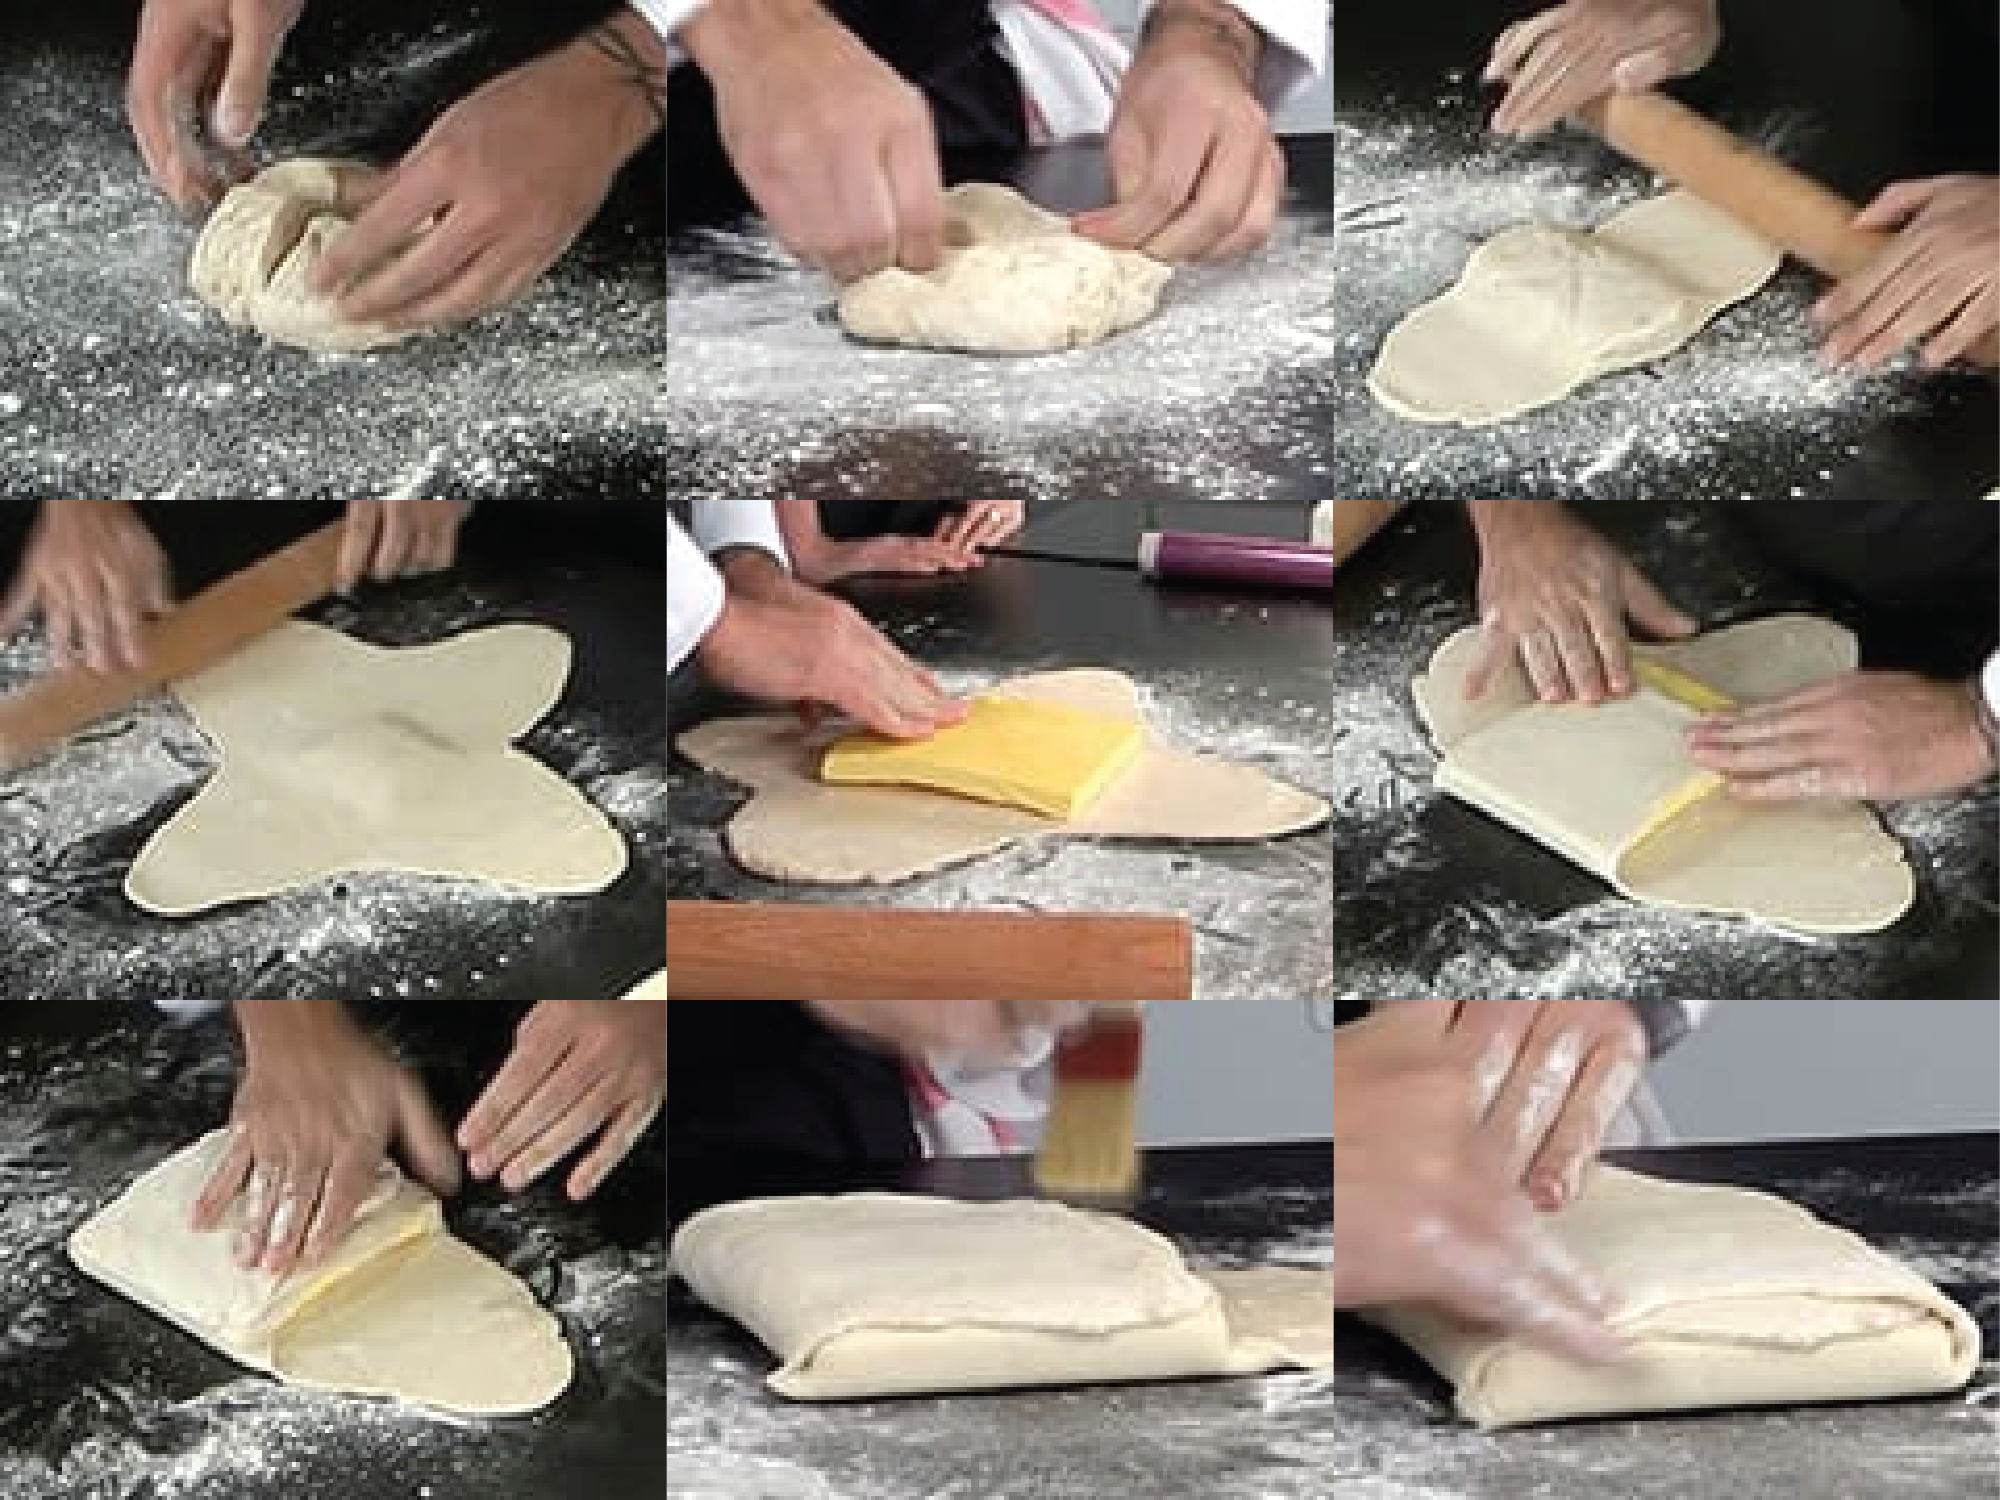
\includegraphics[width=.8\textwidth]{recetas/hojaldre/figures/envoltura.png}
\caption{Así se envuelve la mantequilla con la masa!}
\label{fig:envoltura-hojaldre}
\end{figure}

\begin{figure}
\centering
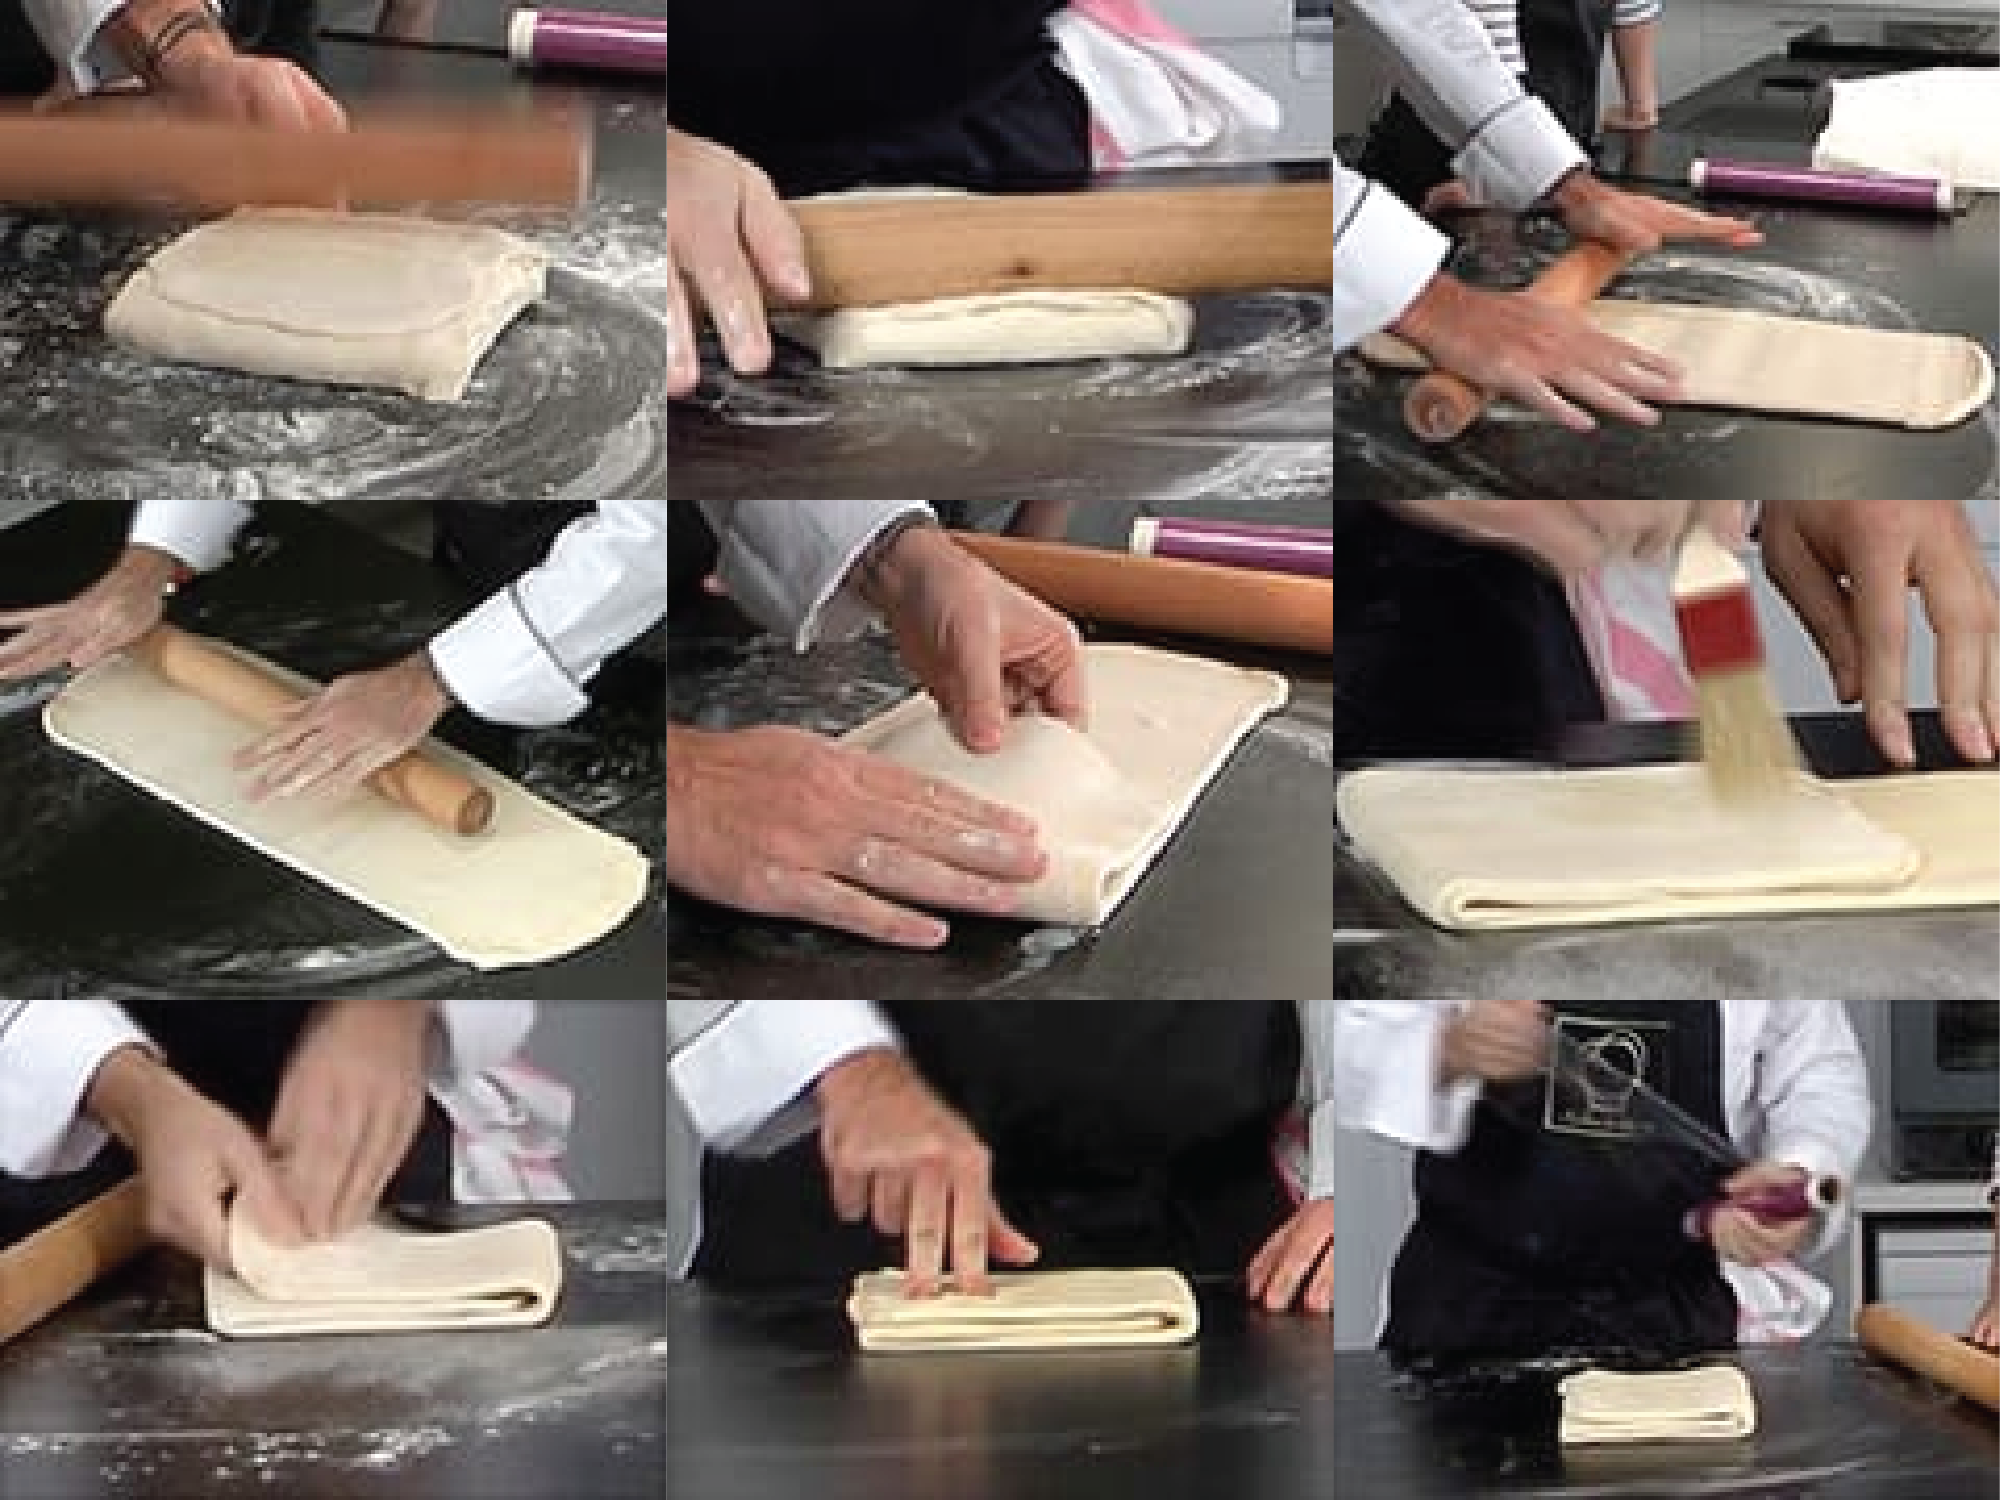
\includegraphics[width=.8\textwidth]{recetas/hojaldre/figures/doblado.png}
\caption{6 de estas!}
\label{fig:doblado-hojaldre}
\end{figure}
\subsection{Masa para croissants}
\label{sec:masa-para-croissants}

Basada en How to make bread por Emmanuel Hadjiandreou y \href{https://www.youtube.com/watch?v=hJxaVD6eAtc}{How To Make Proper Croissants Completely By Hand por Joshua Weissman}

\underline{Ingredientes}

\begin{itemize}
\item 250 gr de harina
\item 20 gr de azucar
\item 1 cucharadita de sal
\item 1$\sfrac{1}{2}$ cucharaditas de levadura
\item 125ml de agua tibia
\item 150 gr de mantequilla
\end{itemize}

\underline{Instrucciones}

\begin{enumerate}
\item Disolver la levadura en el agua tibia.
\item Mezclar la harina, la sal y el azúcar. Sólo hasta que este homogénea, no amasar en este paso.
\item Dejar reposar tapada en el refrigerador por 10 min y amasar jalando una parte de masa y empujándola en medio, 8 veces por todo el perimetro (ver Fig. \ref{fig:amasado-croissant}
\item Repetir el paso anterior, reposo y amasado, 3 veces más (un total de 4 veces).
\item Con la ayuda de papel encerado hacer un cuadrado con la masa de \Sim 15x15cm, y dejar por \Sim 8hrs en el refrigerador.
\item Con la ayuda de papel encerado formar un rectángulo de mantequilla homogéneo de \Sim 10x10cm.
\item Envolver la mantequilla con la masa como se muestra en la Fig. \ref{fig:envoltura-croissant} y dejarla reposar envuelta 1hr en el refrigerador.
\item Estirar un un rodillo como se muestra en la Fig. \ref{fig:doblado-croissant}, y doblar en tres. Trabajar sobre una superficie enharinada. Dejar reposar envuelta en el refrigerador por lo menos 30 min (más si se vuelve difícil de estirar).
\item Repetir el paso anterior 2 veces más (3 en total), girando la masa 90deg cada vez.
\item Dejar reposar envuelta en el refri por lo menos una hora antes de usar. 
\end{enumerate}

\begin{figure}
\centering
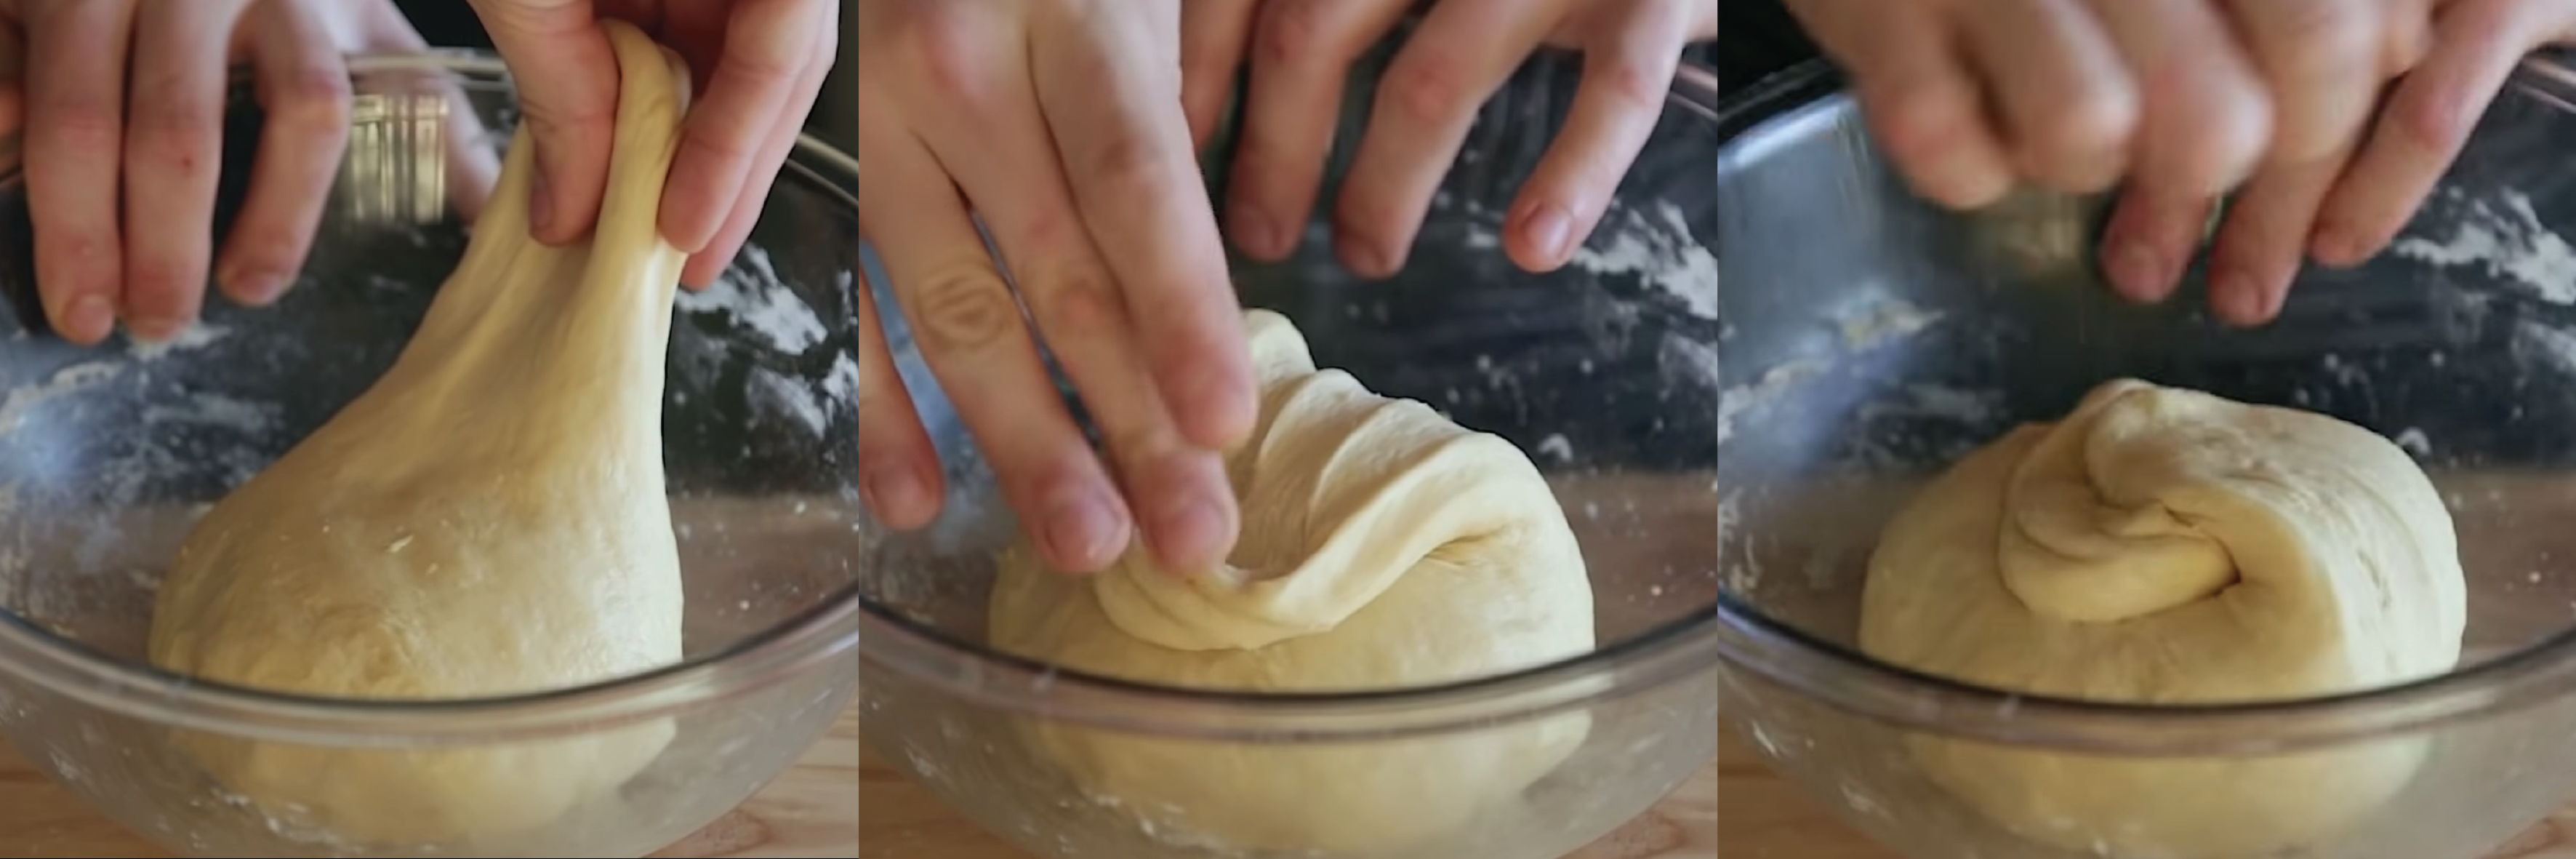
\includegraphics[width=1\textwidth]{recetas/croissants/figures/amasado-croissant.png}
\caption{Así se amasa la masa, 4 de estas! La de la imagen esta amarilla porque le añadieron huevo.}
\label{fig:amasado-croissant}
\end{figure}


\begin{figure}
\centering
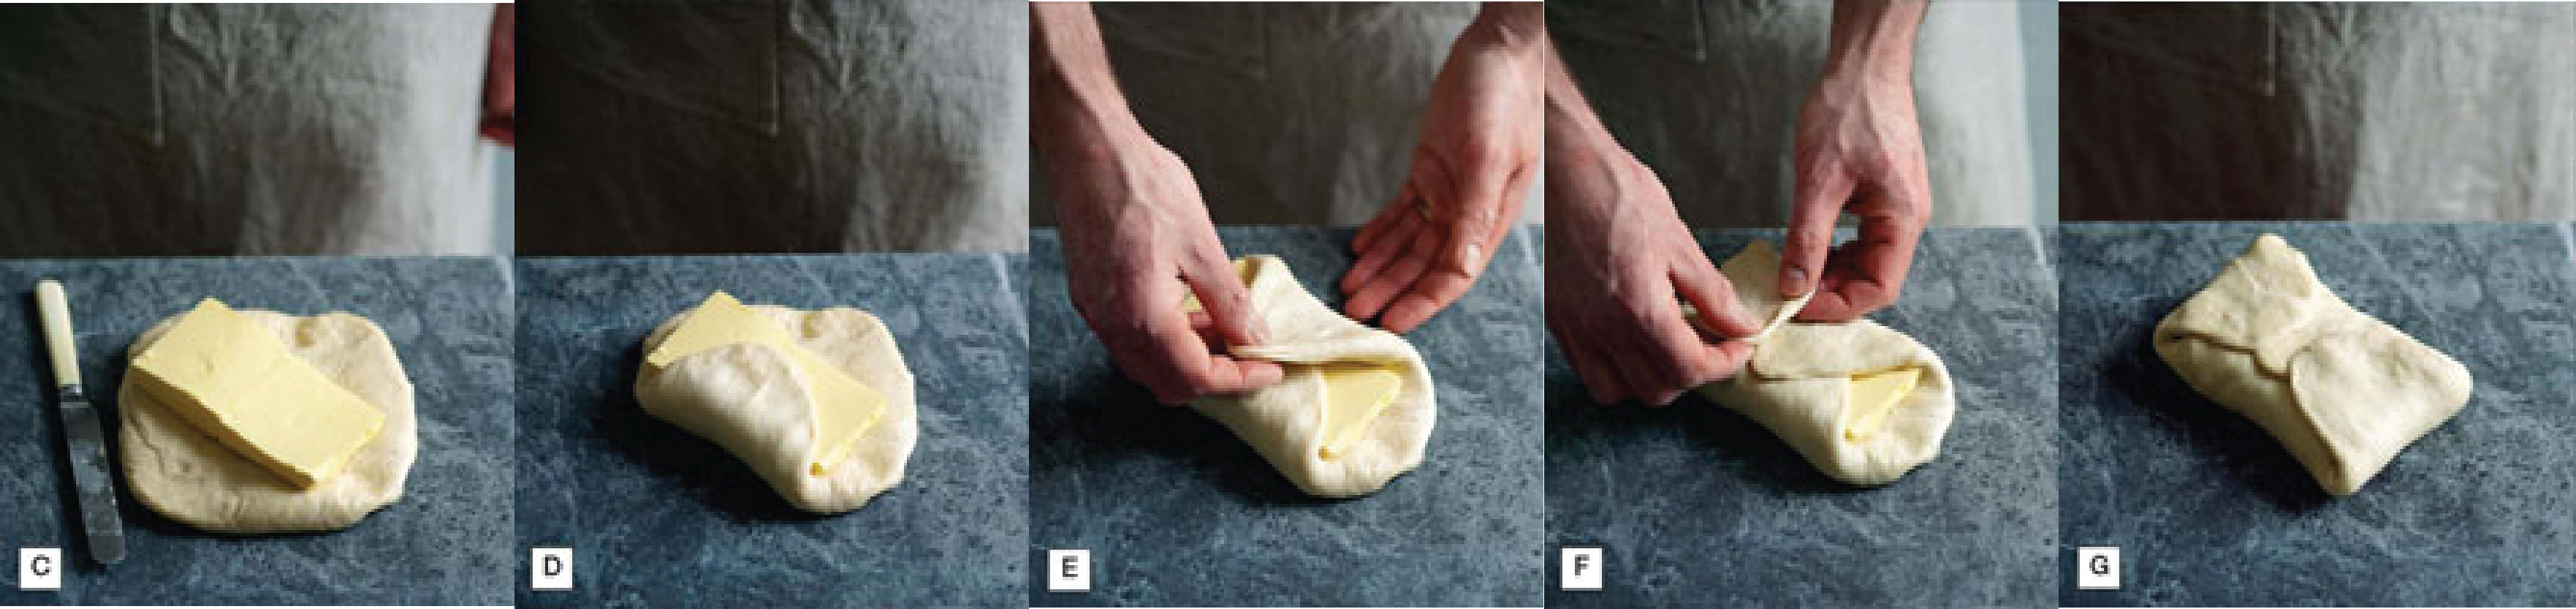
\includegraphics[width=1\textwidth]{recetas/croissants/figures/envoltura-croissant.png}
\caption{Así se envuelve la mantequilla! A mí me gustan más los cuadrados...}
\label{fig:envoltura-croissant}
\end{figure}

\begin{figure}
\centering
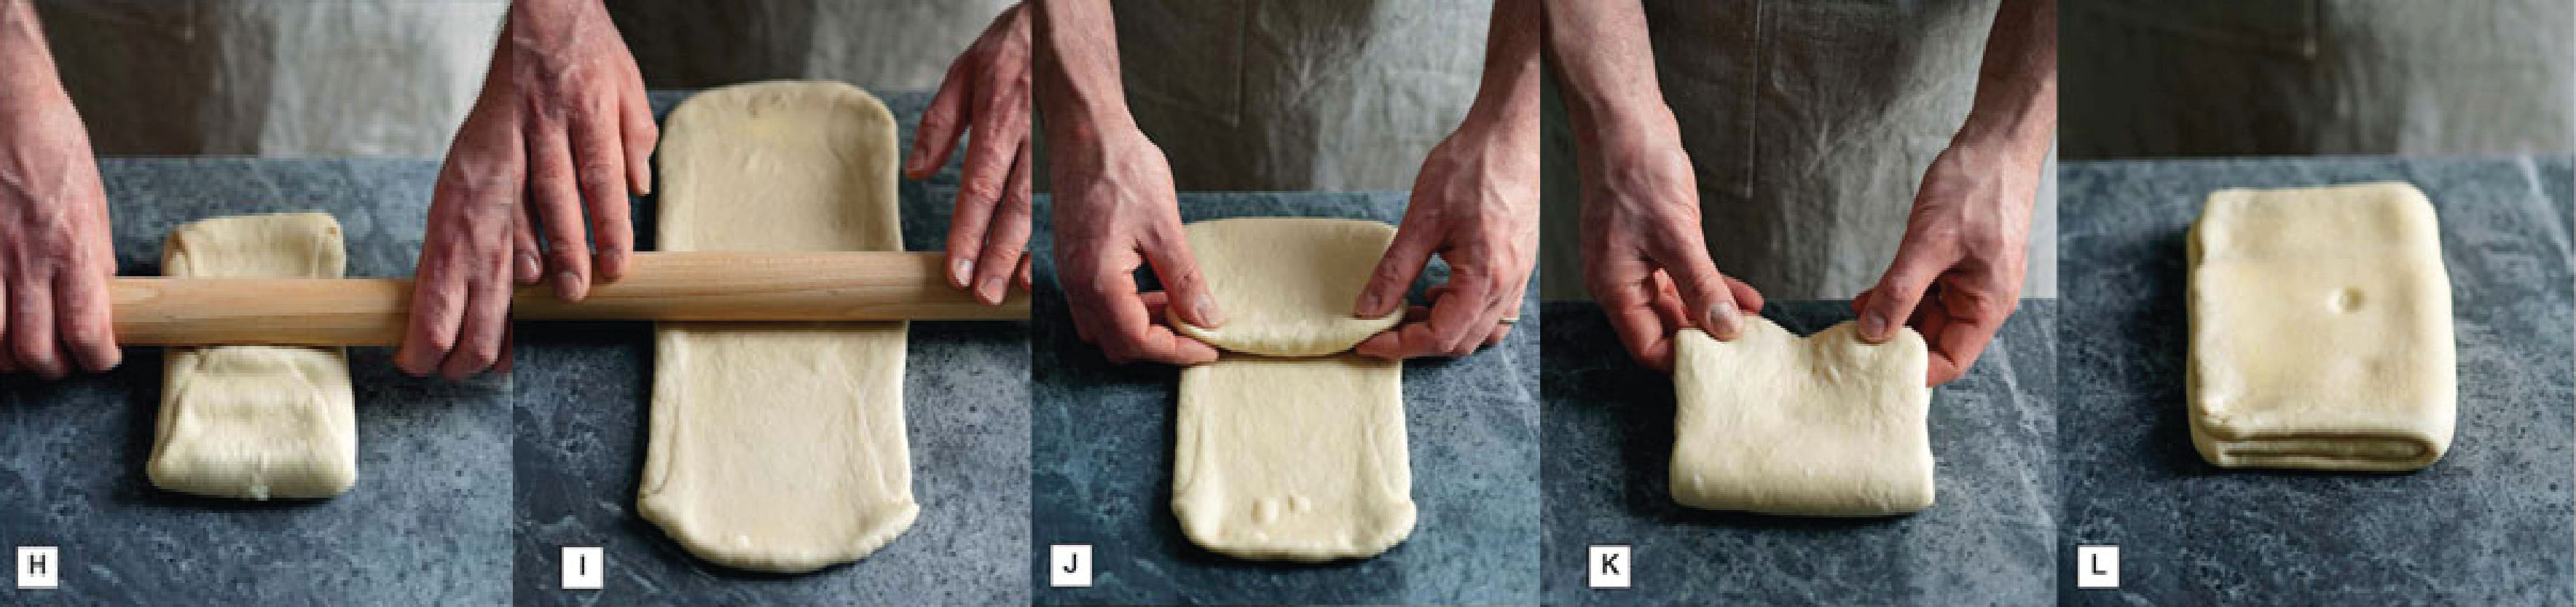
\includegraphics[width=1\textwidth]{recetas/croissants/figures/doblado-croissant.png}
\caption{3 de estas!}
\label{fig:doblado-croissant}
\end{figure}
\subsection{Puerquitos de piloncillo}
\underline{Ingredientes}
\begin{itemize}
\item 500 gr de harina blanca ($\sim 3 2/3$ de taza)
\item 250 gr de piloncillo
\item 1 1/2 taza de agua (360 ml)
\item 3 clavos de olor
\item 2 huevos a temperatura ambiente
\item 1/2 taza de manteca vegetal ($\sim$ 75 gr)
\item 1 cucharada de polvo para hornear ($\sim 9$ gr)
\item 1 cucharadita de bicarbonato de sodio ($\sim 6$ gr)
\item 1 cucharadita de levadura instant\'anea ($\sim 3$ gr)
\item 1 pizca de sal molida
\item 1 cucharadita de a\'uzcar blanca
\item 1/4 de cucharadita de canela en polvo
\item 3 cucharadas de agua ($\sim 30$ ml)
\item 1 cucharadita de extracto de vainilla
\item 1 molde en forma de puerquito

\end{itemize}

\underline{Instrucciones}

\begin{enumerate}
\item Hacer un jarabe. Mezclar la taza y media de agua con el piloncillo, el clavito de holor y la canela en polvo y ponerlo a hervier a fuego alto y mezclar por 15 minutos. Dejar a enfriar. 
\item Poner a fermentar la levadura. Disolver la levadura , la cucharadita de azucar y 1 cucharada de harina en 3 cucharadas de agua tibia. Dejar reposar hasta que duplique su tamaño. 
\item Mezclar la harina con el bicarbonato y el polvo para hornear. 
\item Romper los huevos en recipientes separados. Uno es para barnizar y el otro es para la masa. Batir el huevo para barnizar. 
\item Una vez que se enfríe el jarabe colarlo. Deben salir aproximadamente 1 1/4 de taza o 300 ml
\item Mezclar la harina con la manteca vegetal hasta que esté bien integrada. 
\item Agregar el resto de los ingredientes: huevo, jarabe, sal y levadura. Y amasar aproximadamente por 5 minutos. La masa es bastante aguadita, es normal, no agregar mucha más harina. 
\item Poner la masa en un recipiente tapado y dejar reposar en el refri por 10 minutos. 
\item Engrasar y enharinar 2 charolas 
\item Extender la masa en hasta que quede de aproximadamente 2 cm de grosor. Usar harina para que no se pegue. 
\item Cortar cochinitos. 
\item Retirar el exceso de masa y colocar los puerquitos en charolas engrasadas y enharinadas. 
\item Incorporar el exceso de masa en una bolita (con cuidado de no amasar mucho) y volver a extender para cortar más puerquitos. 
\item Barnizar los puerquitos con el huevo batido
\item Hornear a 180 $^\circ$C o $350^\circ$F hasta que estén doraditos. 
\end{enumerate}

\subsection{Trenza de nuez}

Basada en: \href{http://www.lacocinamexicanadepily.com/2016/12/trenza-de-hojaldre-rellena-de-queso-crema-nuez-y-miel/}{Trenza de hojaldre rellena de queso crema y nuez - La cocina mexicana de Pily}. Cambié la masa de hojaldre por masa de croissant para mejorar la textura, inspirado por la trenza de almudevar.

\underline{Ingredientes}

\begin{itemize}
\item 550 gr de \hyperref[sec:masa-para-croissants]{masa para croissants}
\item 1 paquete de queso crema (8oz, 227gr) a temperatura ambiente
\item $\sfrac{1}{3}$ de taza de azucar
\item 200 gr nuez picada
\item \Sim 4 cucharadas de miel
\item Mantequilla para la charola.
\end{itemize}

\underline{Instrucciones}

\begin{enumerate}
\item Mezclar el queso con el azúcar
\item En una superficie enharinada estirar la masa hasta formar un rectángulo de \Sim 30x75 cm.
\item Con la ayuda de una manga de repostería y una espátula poner una capa de queso con azúcar sobre la masa.
\item Esparcir la nuez sobre el queso.
\item Enrollar todo a lo largo.
\item Cortar el rollo en dos a lo largo.
\item Trenzar las dos mitades, enrollandolas una sobre en la otra, con la parte abierta hacia arriba.
\item Pasar a una charola engrasada y hacer un círculo, tratando de acomodar lo mejor posible las orillas.
\item Dejar reposar por \Sim 1hr hasta que cada capa de masa doble su grosor
\item Hornear a 180 C (350 F) por \Sim 40 min (hasta que esté dorada por completo).
\end{enumerate}

\subsection{Helado de tequila}
\underline{Ingredientes}
\begin{itemize}
\item 1 taza de leche entera
\item $3/4$ de taza de crema para batir
\item 3 yemas de huevo
\item $1 1/2$ caballitos de tequila (o al gusto)
\item 1 pedacito de c\'ascara de lim\'on
\item $1/3$ de taza de az\'ucar blanca

\end{itemize}

\underline{Instrucciones}

\begin{enumerate}
\item Meter el contenedor fr\'{\i}o al congelador al menos 24 horas antes de hacer el helado.
\item Reservar $1/2$ caballito de tequila
\item Batir las llemas de huevo con la leche y la crema.
\item Añadir el az\'ucar, la c\'ascara de lim\'on y un caballito de tequila a la mezcla y poner a cocer a fuego lento en la estufa. 
\item Revolver la mezcla constantemente con un batidor de globo para evitar que se pegue al fondo o que se formen cuajos. Hay que tener mucho cuidado tambi\'en de que no hierva la mezcla para que no se corte. 
\item Una vez que espese un poco (despu\'es de approx 10 min en la estufa) colar y vertir en un recipiente.
\item Una vez que est\'a lista la mezcla agregar medio caballito extra de tequila (o m\'as) para obtener un sabor a tequila m\'as intenso y alcoh\'olico.
\item Dejar reposar la mezcla al menos 3 horas para que espese un poco m\'as antes de poner en la heladera. 
\item Mientras la mezcla reposa meter un recipiente al congelador donde pueda caber todo el helado para que cuando est\'e listo no se derrita al sacarlo de la heladera.
\item Meter la mezcla en la heladera y dejar que se bata $\sim20$ minutos o hasta que est\'e de buena consistencia.
\item Transferir al contenedor que estaba en el congelador y dejar enfriar unas horas para que se termine de solidificar el helado. 

ctodos ingredientes en una olla y poner a cocer a fuego lento en la estufa. 

\end{enumerate}



\section{Salsas}
\subsection{Salsa roja taquera}

\underline{Ingredientes}
\begin{itemize}
\item 4 tomates
\item \Sim 3 dientes de ajo
\item \Sim 20 chiles de árbol
\item \Sim 1 cucharadita de sal
\item \Sim $\sfrac{1}{8}$ de cebolla
\item Aceite vegetal
\end{itemize}

\underline{Instrucciones}
\begin{enumerate}
\item Asar los tomates en un sarten.
\item Dorar los dientes de ajo y los chiles en aceite. Se calienta el aceite, se apaga la flama y después se echan.
\item Licuar todo (sin el aceite). Usar pulsaciones para que quede como martajado.
\item Hervir por unos minutos para que quede más espesa.
\end{enumerate}

\subsection{Salsa verde taquera}

Basada en: \href{https://www.youtube.com/watch?v=sSBfWMCO508}{Easy Recipes, * Chef-roger style *
 - como hacer salsa verde, taquera, Receta \#104, como hacer salsa verde} \\

\underline{Ingredientes}
\begin{itemize}
\item \Sim 5 chiles verdes
\item $\sfrac{1}{2}$ kg de tomate verde
\item 2 dientes de ajo
\item 1 cebolla chica
\item 1 manojo de cilantro
\item Sal al gusto (\Sim 1 cucharada)
\end{itemize}

\underline{Instrucciones}
\begin{enumerate}
\item Cocer los tomates, los dientes de ajo y la mitad de la cebolla hasta que los tomates cambien de color.
\item Licuar
\item Picar el cilantro y el resto de la cebolla
\item Añadir a la salsa junto con la sal.
\end{enumerate}

\subsection{Salsa verde aguacate y tomate}

\underline{Ingredientes}

\begin{itemize}
\item 5 tomatillos cocidos
\item 1 aguacate
\item 1 rebanada de cebolla ($\sim$30gr)
\item $\sfrac{1}{4}$ cucharadita de ajo en polvo
\item Chile verde o jalapeño al gusto ($\sim$ 2 chiles verdes)
\item $\sfrac{1}{4}$ cucharadita de sal
\item $\sfrac{1}{4}$ de taza de cilantro
\item Limon al gusto ($\sim$ 1 lim\'on grande)
\end{itemize}

\subsubsection{Salsa pizza}

\underline{Ingredientes}

\begin{itemize}
\item 130gr ($\sfrac{1}{3}$ de taza) de pasta de tomate
\item 360gr  (1 $\sfrac{1}{2}$ de taza) de tomates enlatados sin semillas y drenados
\item 2 cucharadita de aceite de oliva
\item Oregano al gusto ($\sim\sfrac{1}{2}$ cucharadita)
\item Sal al gusto ($\sim\sfrac{1}{2}$ cucharadita)
\item Ajo en polvo al gusto ($\sim\sfrac{1}{2}$ cucharadita)
\item albahaca al gusto ($\sim$ 5 hojas)
\end{itemize}

\subsection{Salsa tortas ahogadas picosa}

\underline{Ingredientes}
\begin{itemize}
\item 25 chiles de \'arbol secos
\item \sfrac{1}{4} cucharaditas de pimienta
\item 1 cucharada de vinagre de manzana
\item \sfrac{1}{2} taza de agua (donde se cocieron los chiles)
\item \sfrac{1}{2} cucharadita de sal
\end{itemize}

\underline{Preparación}
\begin{enumerate}
\item Cocer los chiles secos ($\sim$5min en agua hirviendo)
\item Licuar los chiles con todo y semilla, con una agua de donde se cocieron y el resto de los ingredientes.
\item Colar
\item Usualmente se le agrega medios aros de cebolla.
\end{enumerate}

\subsection{Salsa tortas ahoagadas de tomate}

\underline{Ingredientes}
\begin{itemize}
\item 1 kg de jitomate
\item \sfrac{1}{2} cucharaditas de comino
\item 2 cucharaditas de oregano
\item 3 dientes de ajo
\item \sfrac{1}{4} de cebolla ($\sim$25 gr)
\item \sfrac{1}{4} cucharaditas de pimienta molina
\item 1 tsps de sal
\end{itemize}

\underline{Preparaci\'on}
\begin{enumerate}
\item Cocer los tomates hasta que revienten.
\item Licuar todo.
\item Colar
\end{enumerate}

\subsection{Salsa macha}

\underline{Ingredientes}
\begin{itemize}
\item \SI{50}{gr} de cachuate
\item \Sim 4 dientes de ajo
\item \SI{15}{gr} de chiles de árbol
\item \SI{25}{gr} de chile morita
\item \SI{1}{cucharadita} de sal
\item \SI{2}{cucharadas} de ajonjoli
\item \Sim $\sfrac{1}{4}$ de cebolla
\item \Sim 1 taza de aceite vegetal
\end{itemize}

\underline{Instrucciones}
\begin{enumerate}
\item Freir las cebollas en el aceite hasta que esten transparentes.
\item Freir los ajos hasta que esten dorados.
\item Dorar los chiles, sin quemarlos.
\item Freir los cachuates hasta que esten dorados
\item Apagar el fuego y echar el ajonjolí.
\item Licuar todo, incluyendo el aceite. 
\end{enumerate}


\section{Sopas}
\subsection{Caldo tlalpeño}
\textbf{Ingredientes}
\begin{itemize}
\item 6 tazas de agua
\item 1 chile chipotle (o al gusto)
\item 1 cucharadita de sal
\item \sfrac{1}{4} de cucharadita de pimienta
\item 120 gr de pechuga de pollo
\item 2 zanahorias cocidas
\item 2 aguacats
\item 1 lim\'on (o al gusto)
\item 160 gr de garbanzo cocido
\item 160 gr de arroz blanco cocido
\item 250 gr de queso panela
\end{itemize}

\textbf{Instrucciones}
\begin{enumerate}
\item Se coce la pechuga. Se cuela el agua pero no se tira.
\item Licua el agua, el chipotle, la sal y la pimienta.
\item Se desmenuza la pechuga.
\item Se agrega el resto y se calienta.
\end{enumerate}

\subsection{Sopa de hongos de Luis}
\underline{Ingredientes}
\begin{itemize}
\item \sfrac{1}{2} kilo de hongos (e.g. baby bella, shitake,  oyster)
\item 1\sfrac{1}{2} jitomates huaje o equivalente
\item \sfrac{1}{4} de cebolla
\item 1 cucharada de aceite
\item 3 dientes de ajo
\item \Sim 1 cucharadita de sal
\item Epazote, perejil, cilantro u oregano al gusto
\item \Sim 2 tazas de agua
\end{itemize}

\underline{Instrucciones}
\begin{enumerate}
\item Licuar el jitomate, la cebolla y el ajo
\item Sofreir en el aceite hasta que se pierda la mayor parte del agua
\item Agregar la sal y las especias.
\item Agregar los hongos y cocer a fuego medio hasta que comiencen a soltar agua.
\item Agregar el agua hasta que casi tape los hongos
\item Hervir a fue alto hasta que el caldo tenga la consistencia adecuada.
\end{enumerate}

\subsection{Sopa de tomate}

Basada en: \href{https://happyhooligans.ca/best-homemade-tomato-soup-recipe/}{Tomato soup from fresh tomatoes - happy hooligans}. \\

\underline{Ingredientes}

\begin{itemize}
\item 3 cucharadas de mantequilla
\item 2 cucharadas de aceite de oliva 
\item 1 cebolla
\item 10 tomates
\item 3 dientes de ajo
\item \num{\sim1/4} de cucharadita de sal 
\item 10 ramitas de tomillo fresco
\item 1 ramita de romero
\item 25 horas de albahaca. 
\item 1 cucharada de arroz
\end{itemize}

\underline{Instrucciones}

\begin{enumerate}
\item Calentar la mantequilla y el aceite a fuego medio.
\item Agregar la cebolla en tiras, la sal, el tomillo, el romero y el ajo.
\item Cocinar tapado a fuego medio por \SI{\sim30}{min}, hasta que la cebolla este suave. Menear ocasionalmente. 
\item Agregar el tomate partido en trozos, el arroz y las hojas albahaca.
\item Cocinar destapado a fuego medio por \SI{\sim 30}{min}, hasta que alcance que la mayor parte del agua se haya evaporado.
\item Remover los palitos de las ramitas de tomillo.
\item Licuar a alta velocidad hasta que este homogeneo.
\end{enumerate}


\section{Vegetariano}
\subsection{Bisteck molido}
\textbf{Ingredientes}
\begin{itemize}
\item \sfrac{1}{2} litro de agua
\item 1 cucharada de oregano molido
\item 1 cucharada de sal
\item 1 cucharadita de ajo molido
\item $\sfrac{1}{4}$ de cebolla picada finamente
\item \sfrac{1}{4} de cucharadita de pimienta
\item \sfrac{1}{8} de cucharadita de comino molido
\item 100 gr de soya texturizada
\item 1 cucharada de aceite vegetal
\end{itemize}

\textbf{Instrucciones}
\begin{enumerate}
\item Se pone todo exepto la soya y el aceite en una cacerola hasta que hierva
\item Se agrega la soya y se apaga la flama. Dejar reposar por 5 min.
\item Con un colador y un cucharon exprimir la soya lo m\'as que se pueda. 
\item Se fr\'ie la soya preparada.
\end{enumerate}


\section{Bebidas}
\subsection{Caipirinha}

\textbf{Ingredientes}
\begin{itemize}
\item 1 taza de hielo picado
\item 1 limon mediano exprimido y partido
\item $\sfrac{1}{2}$ cucharada de azucar
\item 3 cucharadas de cachaca
\end{itemize}


\section{Tiempos}
\subsection{Olla de presi\'on}

\begin{table}[H]
  \begin{tabular}{l | c | l}
    & Tiempo (min) & Notas \\
    \hline
    Lengua     & 50 &  \\
    Lomo    & 15-20  & Dependiendo de la consistencia deseada \\
    Bistec        & 15-20  & Dependiendo del grosor (3-15 cm)
  \end{tabular}
  \end{table}


\end{document}

